\documentclass[11pt,landscape]{article}
\usepackage[a3paper]{geometry}
\usepackage{graphicx}
\usepackage{fancyhdr}
\usepackage{multirow}
\usepackage{multicol}
\usepackage{textcomp}
\usepackage{gensymb}
\usepackage{amsmath, amssymb}
\usepackage{float}
\usepackage{wrapfig}
\usepackage[hidelinks]{hyperref}
\usepackage[parfill]{parskip}
\usepackage{glossaries}
\usepackage{amsmath}
\usepackage{mdframed}
\usepackage{caption}
\usepackage{siunitx}
\usepackage{makecell}
\usepackage{pdfpages}
\usepackage[none]{hyphenat}

\newenvironment{Figure}
  {\par\medskip\noindent\minipage{\linewidth}}
  {\endminipage\par\medskip}

\geometry{margin=2cm}

\graphicspath{{./images/}}

\pagestyle{fancy}
\setlength{\headheight}{24pt}
\fancyhead[L]{GDP Group 35}
\fancyhead[R]{Design of a Smart Autonomous Golf Cart Caddy}
\fancyfoot[C]{\thepage}


\begin{document}
\pagenumbering{arabic}
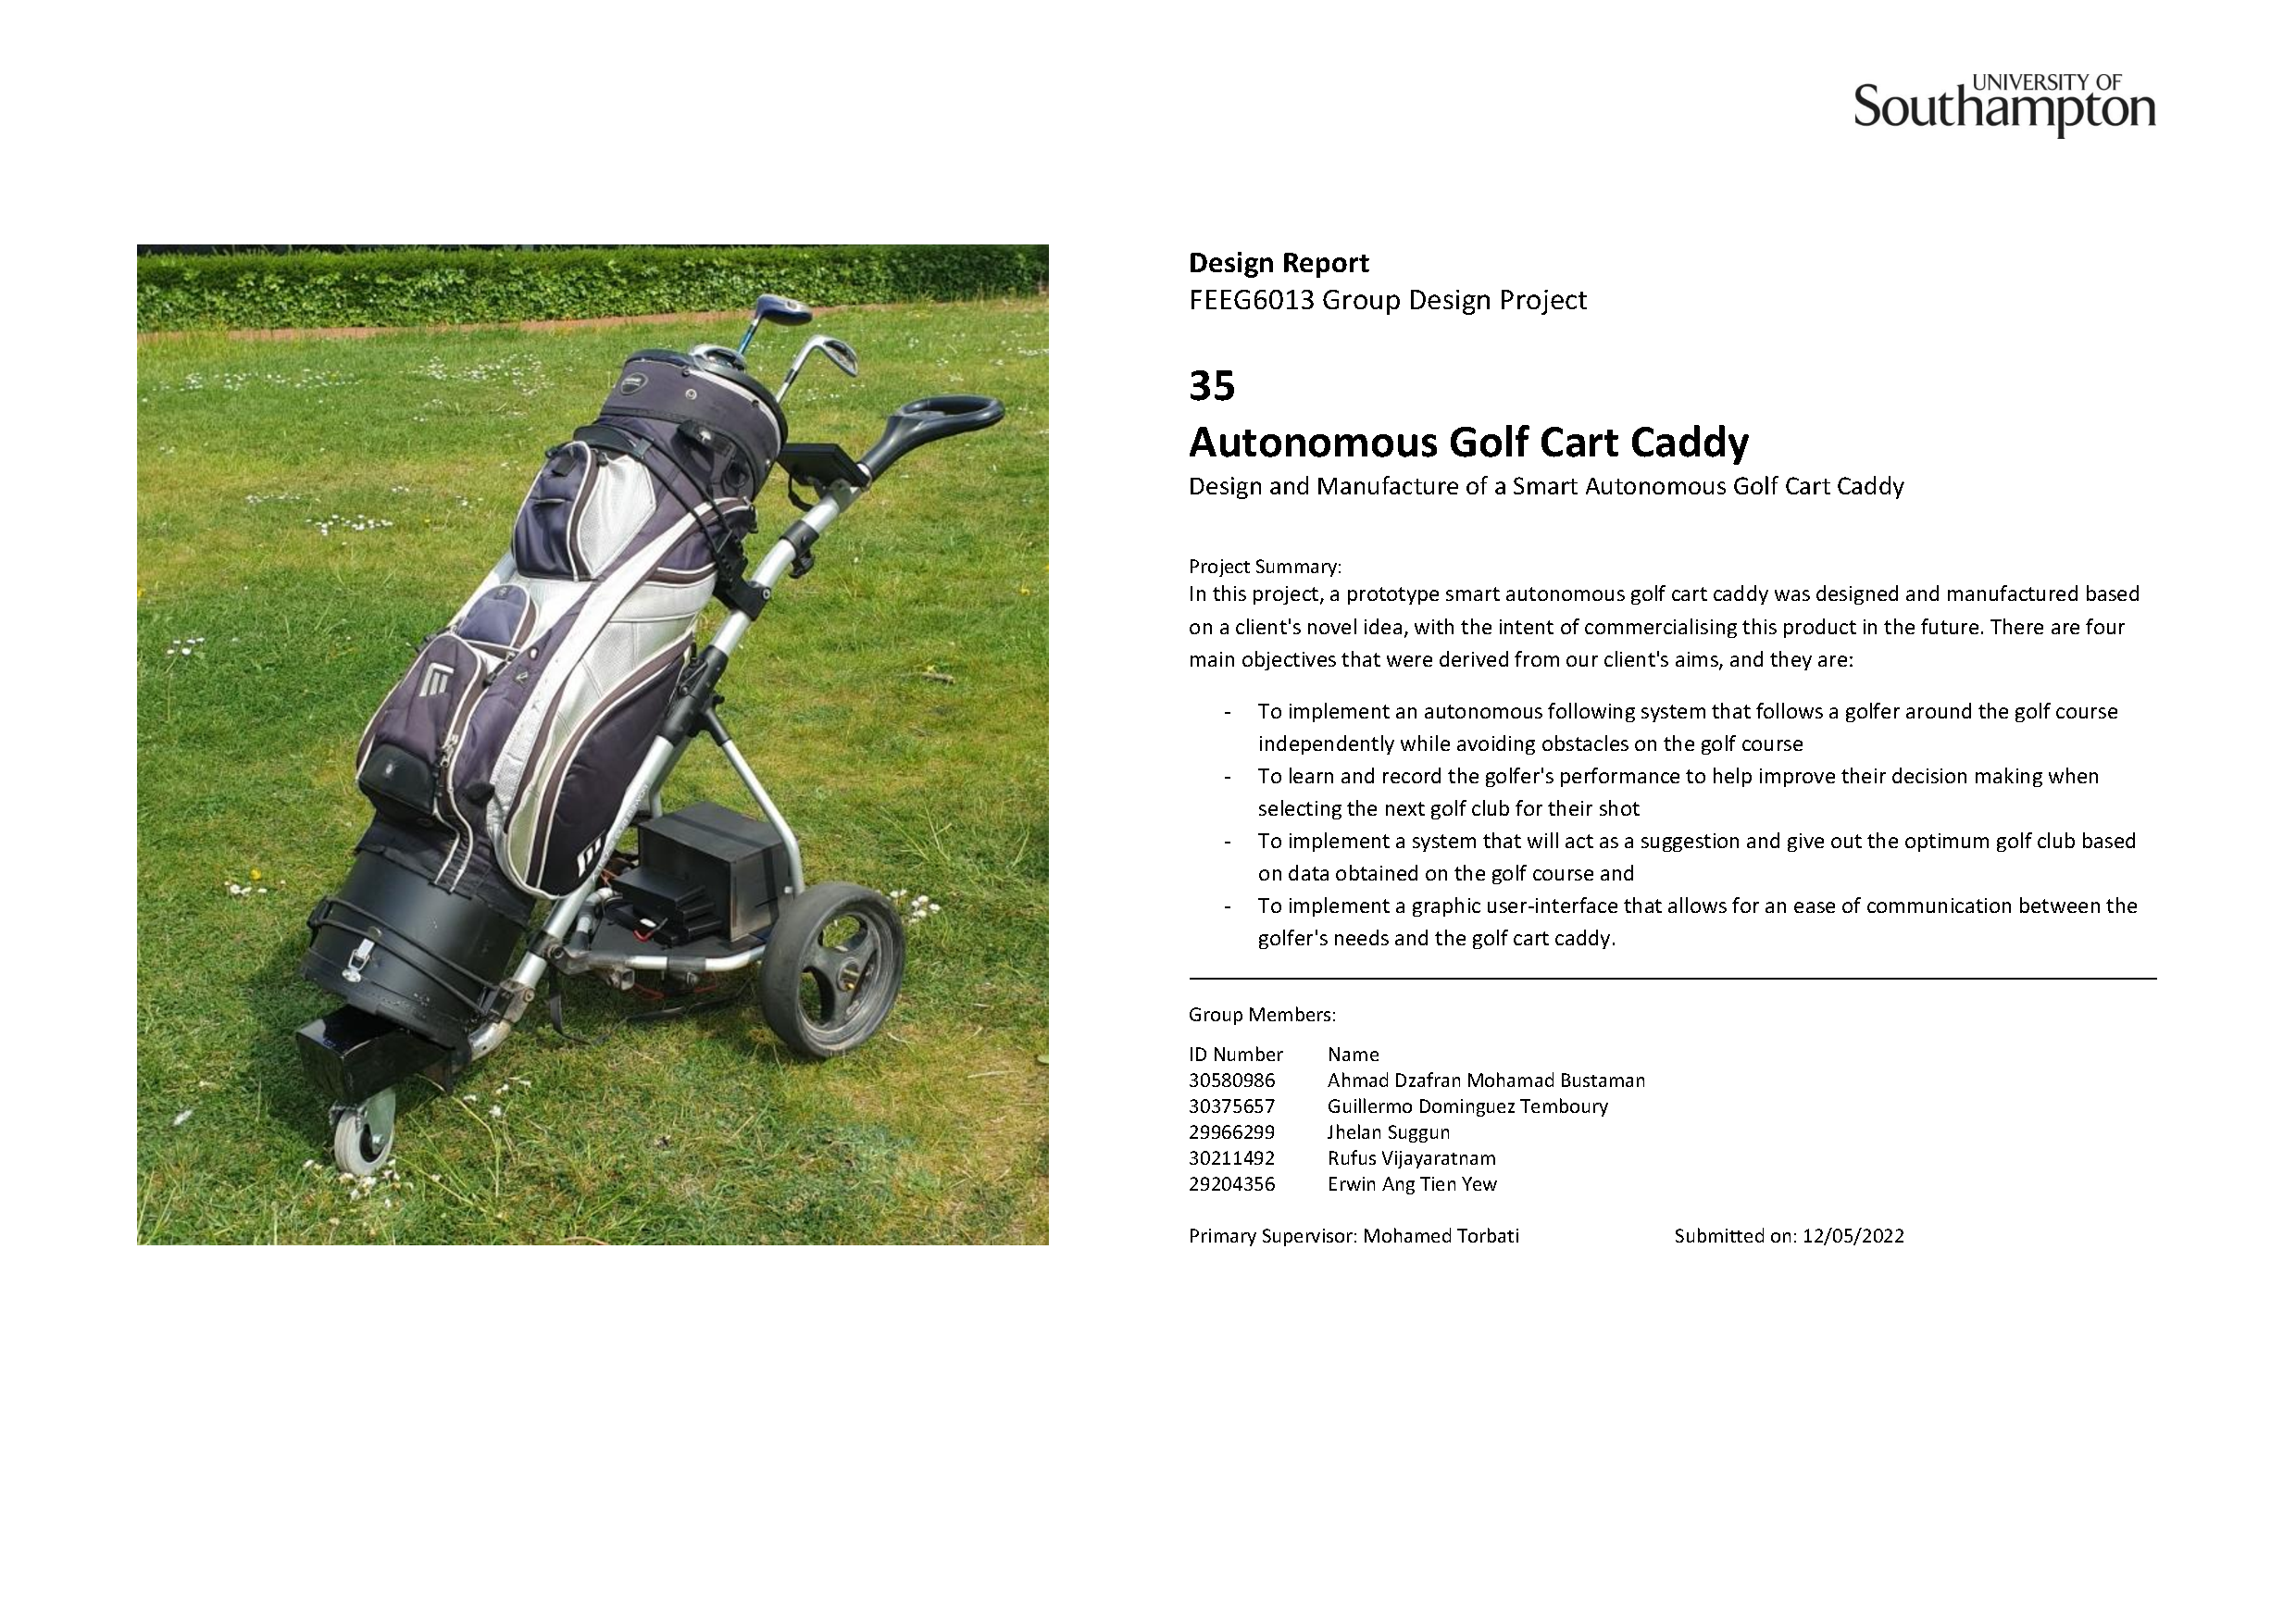
\includepdf{cover.pdf}
\newpage
\begin{multicols}{2}
\tableofcontents
\newpage
\section{Introduction}
Caddy is a person who carries a player's bag and clubs, and gives the player advice
and moral support. In this modern era, mobile robot platforms are not strange concepts
and have been utilised not only for transportation but also have been diversified in
other services such as medical, industrial and even sports. Autonomous golf
caddies are also emerging technologies in the sport. Like typical caddies, they provide
support by carrying the golfer's golf clubs and provide useful information such as
weather forecast and wind trajectory throughout the round of golf. There are typically
two modes of operation provided by current golf cart caddies where it can either
follow the golfer autonomously and remotely, although some type of tracking sensor
is required such as a Bluetooth pod; or through manual control where the
golfer needs to guide the caddy through the golf course using a remote control.
\cite{choi_2020}. These modes are of course interchangeable with the transition
from manual to autonomous and vice versa via an interaction between the
golfer and the golf cart caddy. Recent improvements on the design concepts of
autonomous golf caddies on the market have been made; especially on the autonomous
following. The M5 GPD DHC Trolley for instance, features a rechargeable lithium
battery and secure Bluetooth connectivity remote control that enables the caddy
to follow the golfer independently as long as the remote control is attached on
the golfer and within 50 meters of the golf cart caddy \cite{golf_2022}.

However, such high-end technology leads to the product being very expensive;
this particular product cost £950 thus not being a popular choice for those
who intend to join the sport at the early stages. In addition, although the
golf cart caddy can be independent, needs some guidance as to where it should
go considering that the golf course is full of hazards such as bunkers and lakes.
Although current technologies are capable of supporting the golfer in the ways
previously mentioned, there is a lot of potential in improving the golf cart caddy.
Experienced golfers would have better understanding of their rounds and better
intuitions to make decisions on which golf clubs would be best used for the
current shot. However, beginner golfers lack experience and would have trouble
in making decisions on the golf course. There is a potential to have the golf
cart caddy to aid them in making decisions based on computational analysis
of their previous shot data, local weather forecast, and wind trajectory. 

Improvements can be made to the current autonomous golf cart caddies so that
it would be more affordable and accessible to the general public while aiding
current golfers with their performance and encourage new talents to the sport. This
project considers the design, manufacture and testing of a prototype Autonomous
Golf Caddy (AGC), with emphasis on these improvements. Although current
regulations do not permit computer aids for professional games as this would be
an unfair advantage, the improvements on this feature could be used
during casual games and training so that golfers could analyse their performance
by comparing it to computational analysis of their games.  

\subsection{Aims}
The concept of this project was proposed by our client, an avid golfer who wishes
to improve his game of golf and hope to present a new product to the market
targeting new talents in golf. Based on the clients requirements and considering
the requirements of the university's Group Design Project (GDP), the team has set
a list of aims prior to the start of the GDP, aligning both stakeholder's
requirements, to achieve at the end of the project: 
\begin{itemize}
    \item Develop a prototype of a smart autonomous golf cart caddy within the budget
    provided by the university that is able to follow the golfer around the golf
    course while avoiding unallowed locations such as the greens, bunkers and
    waters. 
    \item Design the caddy that could offer an optimum golf club to the golfer
\end{itemize}
\vfill\null
\columnbreak

\subsection{Objectives}
After understanding the ideas proposed by our client, the team has identified
several objectives that needs to be fulfilled in order to achieve the aims of
this project: 
\begin{itemize}
    \item Design and implement a system that allows autonomous tracking between
    a golfer and the caddy 
    \item Develop and implement a machine learning algorithm into the caddy that
    will be used to record data from the golfer’s performance 
    \item Design and implement a system that will offer the optimum golf club
    needed for the next shot based on the machine learning algorithm 
    \item Design and develop a User-Interface system so the golfer can interact
    with the AGC
\end{itemize}

\subsection{Resources}
The team was allocated s maximum budget from the university of £850 and was
also supported by our client where the team is provided with golf equipment to
design the project and conduct testing. A full break down of our project
expenditure and funding can be seen in appendix (A). 

\subsection{Team Roles and Work Breakdown}
The team was structured and organised in a way such that everyone's set of skills
could be fully utilised thus making the most out of this project. The team`s
breakdown of roles can be seen below in Table (\ref{tab:roles}). 

\begin{table}[H]
    \begin{center}
        \resizebox{\columnwidth}{!}{%
        \begin{tabular}{|l|l|l|}
            \hline
            \textbf{Team Member} & \textbf{Primary Role} & \textbf{Secondary Role} \\ \hline
            Ahmad Dzafran bin Mohamad Bustaman & Course data gathering & GUI \\ \hline
            Guillermo Dominguez Temboury & Machine learning & Electronics \\ \hline
            Jhelan Suggun & Mechanical design and manufacturing & Testing \\ \hline
            Rufus Vijayaratnam & \makecell{Autonomous control software \\ Motor and controller software} & Electronics \\ \hline
            Erwin Yew & Design and manufacture & Testing \\ \hline
        \end{tabular}
        }
        \captionof{table}{Team member roles}
        \label{tab:roles}
    \end{center}
\end{table}

\subsection{Ethical and Sustainability Considerations}
An ethical concern pertains to whether or not this newly designed caddy follows
the rules and regulations of golf. Although the implementation of the machine
learning algorithm is not allowed as this would be an unfair advantage in a
professional game, the intention of this feature is focused on training and
encouraging new talents that are keen in joining the sport. Besides that, all of
designs and implementations are acceptable within the rules and regulations.
Additionally, as large amounts of data will be collected on the golfer,
assurances must be made that the data is properly protected if made commercially
available. In terms of sustainability, the usage of a rechargeable lithium
battery encourages greener alternative to energy consumption. Besides that, the
design of the AGC follows standards of current products on the market with
slight adjustments in the dimensions which does not have any significant impact
to the golfer, people around and its surrounding. Since the implementations of
the design and systems are on an existing caddy, this has saved the team a lot
of material resources and cost.  

\subsection{Design Process}
The smart autonomous golf caddy consists of many sub-systems thus requires a
structured and clear design process in order to be successful. The design
process covers all the stages of the design and manufacturing process that the
team followed in order to achieve a reliable and high-quality prototype.

\begin{Figure} 
    \begin{center}
        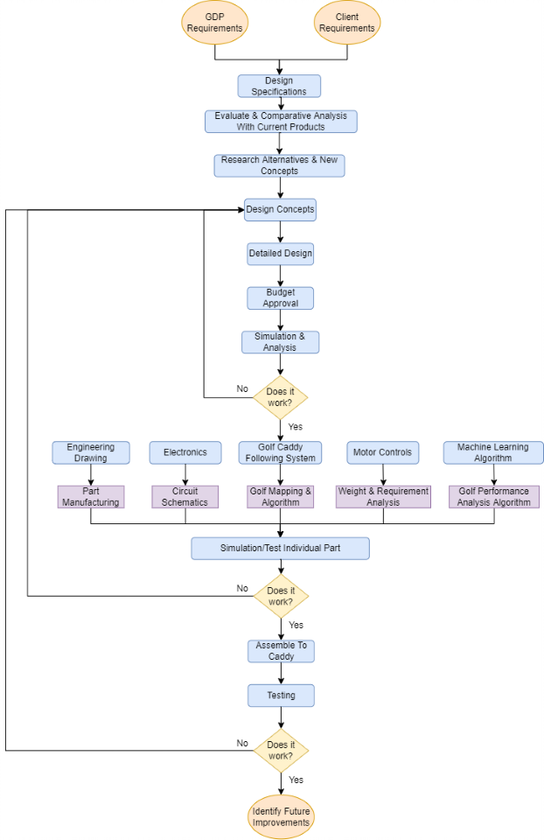
\includegraphics[width=0.8\textwidth]{design_process.png}
    \end{center}
    \captionof{figure}{Flow chart showing our design process}
    \label{fig:design_process}
\end{Figure}


All components of the caddy including its systems were interconnected and thus a
design process flowchart as seen in Fig. (\ref{fig:design_process}), was made to
ensure all the design process was clear and done in a properly manner to obtain
the best result for the project. The design process follows a 5 stage approach.
The first stage consist of defining the problem, brainstorming possible solutions
and exploring new concepts and possibilities for the design of the project. It was
important for the team to cater to the requirements of the client without going
astray of the requirements of the GDP. Initially, the request was to design and
develop a fully functional smart AGC that was commercialisable. However, this
was not possible considering the time and budget allocated for this project by
the GDP stakeholders thus the team proposed to design and develop a functioning
prototype that could be further improved in the future. Next, the team identified
the design specifications of the standard caddy, researched and explored new
features and concepts, and subsequently evaluated and compared the ideas with
current products available on the market. 

The second stage was to select a concept and develop a design proposal. This
stage consist of the team working on their roles and introducing the concepts to the
team and client. Concepts that did not meet the requirements were rejected and
the design proposal were refined during discussions. It was also important to
the team that the client was presented with all the information and ideas in
order to meet the client’s requirements. It was also found very insightful and
helpful as the client gave feedback and other perspectives to consider. 

The third stage was simulation and prototyping. The algorithms and codes for the
machine learning and golf caddy following were develop and simulated. The mechanical
designs, motor controls and electronics were tested based on the design
specifications. All components of the project were simulated or tested
individually to ensure that risk of individual part problems was minimised
before assembly. This process was important to mitigate any risk that could be
hazardous to the team and everyone involved during the prototyping process and
reduce errors that could lead to wastage of resources. 

The fourth stage is assembly and testing. After assembling all individual
components to make the prototype caddy, testing was conducted. The testing
involved the client, as an experienced golfer, to observe and analyse the
functioning of the prototype caddy. The fifth and
final stage is to identify further improvement that could be made to the design.
In the case of this project, this could mean developing and improving the design
to commercialising standards given the necessary time and funding. 

\subsection{Inheritance and Design Changes from Original Golf Caddy}
Although this is a new project within the GDP, the team were given a golf bag
and caddy by the client. The team had to test, redesign and add a significant
amount of hardware, software and electronics to the inherited design. In
addition, the team also added a few innovations relevant to the project’s
aims and objectives. To aid the clarification of this project, Fig.
(\ref{fig:inheritance}) details a diagram of the individual changes made
from the inherited design and developed components. 
\end{multicols}
\newpage

\begin{figure}[H]
    \begin{center}
        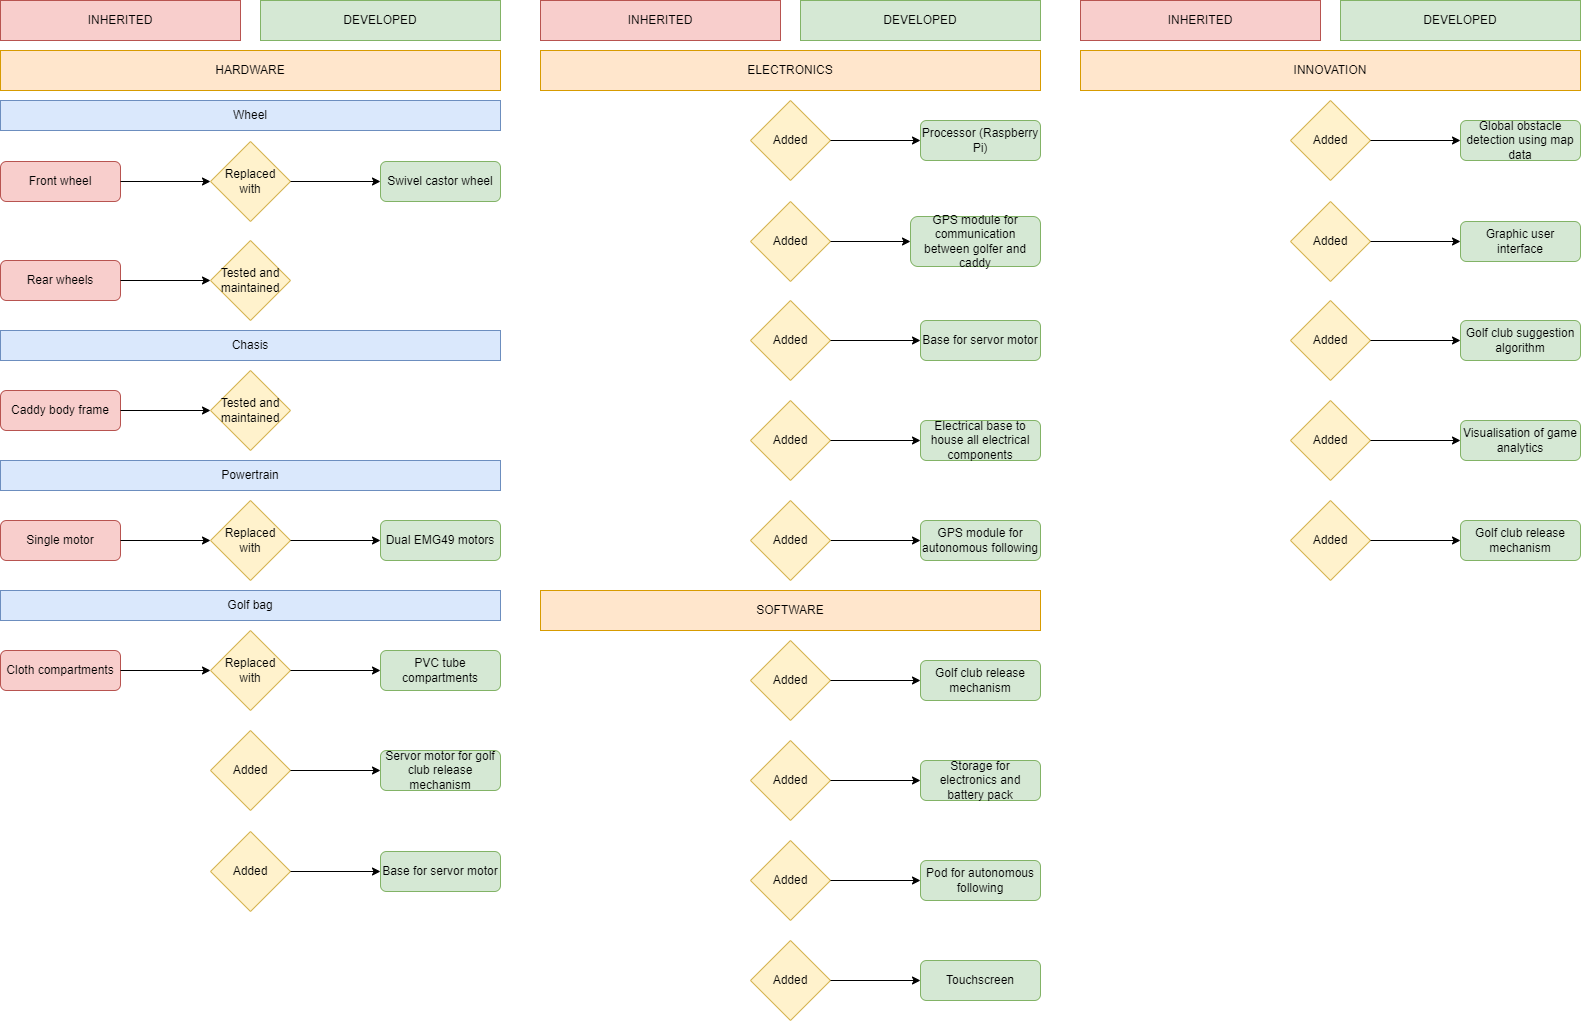
\includegraphics[width=\textwidth]{inheritance.png}
    \end{center}
    \captionof{figure}{Flow chart showing our design inheritance}
    \label{fig:inheritance}
\end{figure}


\newpage

\section{Final Design Proposal}
Shown below in Fig. (\ref{fig:final_proposal}) is the final design for our
prototype AGC. The design, testing and review of all relevant components, systems, and software is
documented through the rest of this report.

\begin{figure}[H]
    \begin{center}
        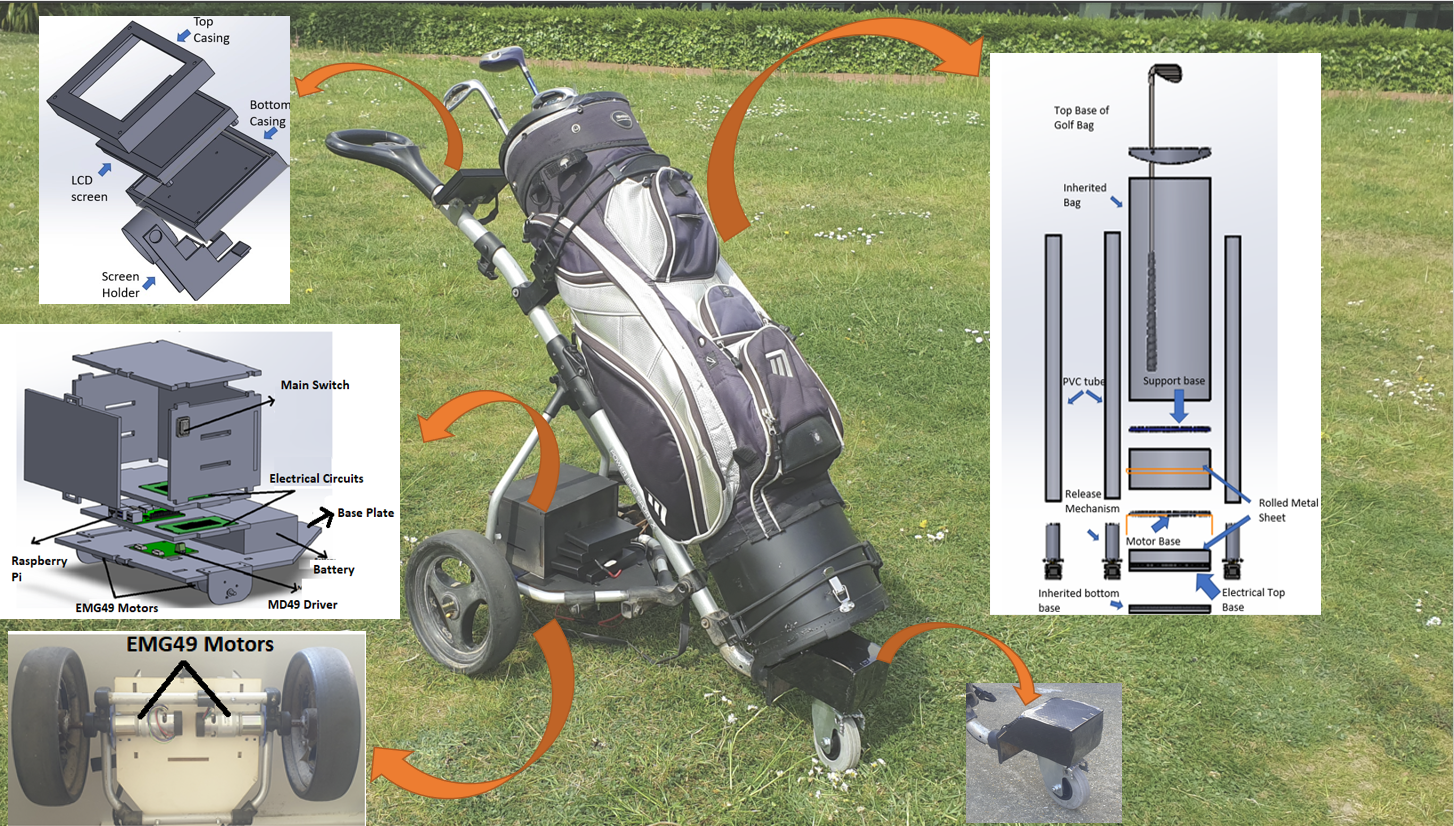
\includegraphics[width=\textwidth]{final_proposal.PNG}
    \end{center}
    \captionof{figure}{Final Design Proposal}
    \label{fig:final_proposal}
\end{figure}

\begin{multicols}{2}

\section{Mechanical Design}
    In this section, several mechanical components that were designed,
    manufactured and implemented are discussed. However, considering the
    grandscale of things, this project only places its proposed design in the
    prototype phase of this novel idea. Therefore, an emphasis was placed on
    achieving the most effective design that will achieve the objectives set out
    at the start of this project whilst making best use of the resources
    available such as manufacturing workshops, material and the inherited
    components from the golf caddy. 
    
    \subsection{Release Mechanism}
    One of the key objectives for this project was to design and implement a
    release mechanism that will raise a golf club as a form of suggestion for
    the golfer’s next shot towards the green, based on a machine learning
    algorithm. This is a novel idea presented by our project advisor and is one
    of the many innovative designs that will be implemented in this project.
    
    \subsubsection{Design Requirement}
    Initially, the workspace that will hold such mechanism had to be identified
    as it will be part of the design requirements before making any prototypes.
    Three feasible locations were considered which were to either be integrated
    in the golf bag, to be integrated on the AGC such that the golf bag
    will rest on top of it, or to be in a separate compartment that will need to
    be attached to the golf bag and AGC. The selected option was for the
    mechanism to be integrated in the golf bag as this reduces the likeliness of
    errors occurring since the mechanism does not have to be removed and
    reconnected after every game from the golf bag. The design requirements are
    listed as follows:
    
    
    \begin{itemize}
    \item Need to lift at least 10 cm above other golf clubs to make it clear
    which club is being suggested
    \item Needs to lift the weight of the golf club
    \item Needs to be lightweight since the golf bag will be carried by the user
    before it is mounted on the caddy
    \item Needs to be a robust design since it will be used multiple times
    during a game
    \item Needs to fit inside the designated workspace that is inside the golf
    bag
    \end{itemize}
    
    \subsubsection{Concept Design}
    Various mechanisms that provides linear translation motion, which are
    desired, were explored. However due to the design requirements, two main
    concept ideas were considered to be the most suitable and they are shown in
    Fig. (\ref{fig:design}).
    
    \begin{Figure}
        \begin{center}
            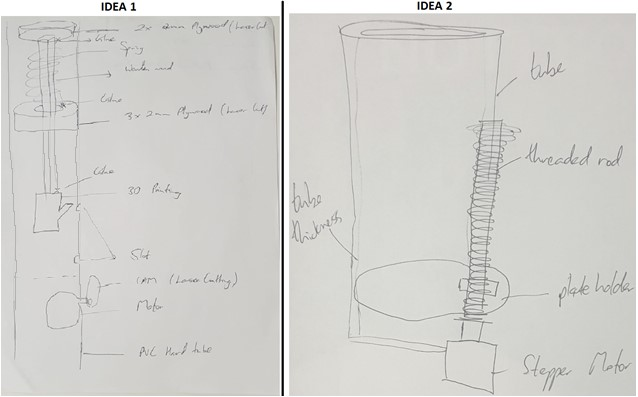
\includegraphics[width=\textwidth]{Figure19.jpg}
            \captionof{figure}{Concept design for release mechanism}
            \label{fig:design}
        \end{center}
    \end{Figure}
    
    Idea 1 consisted of an umbrella type mechanism which uses a compression
    spring, and with the use of a stepper motor and cam, the system can be
    released from a “loaded” state to elevate the component. Idea 2 was more
    innovative as it made use of a similar mechanism that is employed in a linear actuator. In this design, a plate holder is
    attached to a nut and it is placed on a stepper motor with a threaded rod.
    This plate holder is placed within a tube and by using the inner wall of the
    tube as a restriction to prevent the rotation of the nut when the stepper
    motor provides a torque, the plate holder’s only direction of motion can be
    either up or down the tube. Idea 2 was selected as the preferred design of
    choice. The most important reason this option was chosen was that this
    design does not require the user to push down the golf club in order to put
    the system in a “loaded” state compared to Idea 1. It also offers a safer
    and more controlled way to elevate the golf club compared to the spring
    action which will make the golf club jump upon release. Another benefit was
    that there are less parts involved in order to make the whole mechanism
    compared to Idea 1 and therefore there is a less chance for failure to
    occur. To calculate the required torque for the stepper motor, the maximum
    weight of the heaviest golf club that was measured to be 700g, was used in further
    calculations. The torque was calculated, by modelling it mathematically similar to a pulley problem, with the
    formulas shown below in Eqs.(\ref{eq:raising_force} and \ref{eq:raising_torque}).
    
    \begin{center}
        \begin{equation}
            F = W = mg
            \label{eq:raising_force}
        \end{equation}
    \end{center}
    \begin{center}
        \begin{equation}
            T = Fr = Mgr
            \label{eq:raising_torque}
        \end{equation}
    \end{center}
    
    Where $m$ is the mass of the golf club, $g$ is the gravitational
    acceleration constant, and $r$ is the distance from the centre of the plate
    holder (the assumed position of the golf club’s handle) to the centre of the
    threaded rod. A torque value of 0.13 Nm was calculated, however, the closest
    rated torque for a motor that could be obtained was the NEMA 17 stepper
    motor which has an output of 0.42 Nm. This motor was chosen since it allows
    for a safety factor of 3.2, which is appropriate considering the previous
    calculations neglected the friction acting between the nut and the threaded
    rod as well as the fiction between the plate holder and the inner wall of
    the tube. 
    
    
    \subsubsection{Testing and Improvement}
    Idea 2 was then made into a prototype, as shown in Fig. (\ref{fig:release}),
    to test the effectiveness and robustness of the system. 
    
    \begin{Figure}
        \begin{center}
            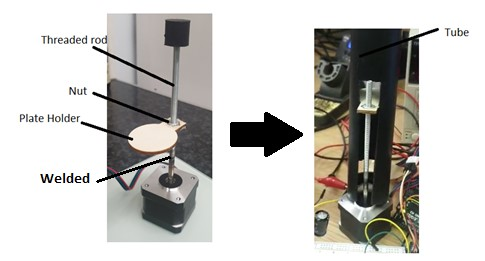
\includegraphics[width=\textwidth]{Figure20.jpg}
            \captionof{figure}{Release Mechanism Prototype}
            \label{fig:release}
        \end{center}
    \end{Figure}
    
    The initial testing of the prototyping demonstrated that the design worked
    well, with a time of 12.7 seconds recorded to lift the golf club by 10 cm.
    However, a serious issue was discovered where the plate holder could get stuck
    within the tube and thereby fail the whole system. Furthermore, there was
    bending observed on the plate holder when the golf club was not perfectly
    placed in the middle of the plate. Another issue was that the time taken for
    the club to be raised was particularly long which is due to the pitch of the
    threaded rod being small. 
    
    In consequence of that, some improvements were
    made to this design. The stepper motor with the threaded rod was changed to
    one with a leadscrew integrated as its shaft and this will decrease the time
    to raise the golf club. A way of mitigating the risk for a system failure
    due to the plate holder getting stuck inside the wall of the tube, was to
    use a cylinder where its lower plate will have the leadscrew nut mounted on
    using nuts and bolts. It was deemed to be a more robust design that can
    easily support the weight of the golf club and with the implementation of
    guiding rails, which are threaded rods in this case, the inner tube walls
    will not be used to restrict the rotating motion of the cylinder. 
    
    This cylinder was manufactured using 3D printing with PLA filament as
    the material. Taking into account the stair stepping effect and porosity
    from 3D printing, the cylinder was made to be sufficiently strong enough to
    hold the maximum weight of a golf club recorded. After incorporating these
    improvements, the calculated time to raise the golf club by 10 cm was
    recorded to be 3.6 seconds which is almost 3.5 times faster than the
    prototype version. The overall weight of this design only amounts to 400g
    per mechanism and since only three release mechanism has been promised to be
    implemented in this project, the total added weight amounts to 1.2 kg which
    is only an 8\% weight increase from an original golf bag weight of 15 kg. 
    
    
    \subsubsection{Final Design}
    The final and proposed design assembly and the built design is shown in
    Figure \ref{fig:release1}
    
    \begin{Figure}
        \begin{center}
            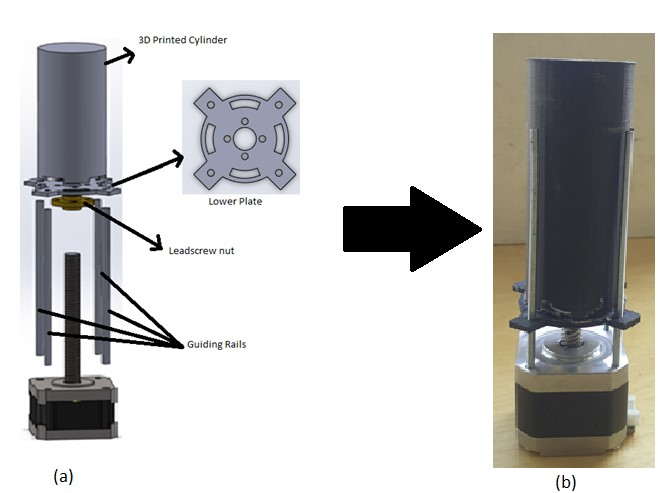
\includegraphics[width=\textwidth]{Figure21.jpg}
            \captionof{figure}{Proposed Release Mechanism (a)Assembly (b)Manufactured Product}
            \label{fig:release1}
        \end{center}
    \end{Figure}
    
    
\end{multicols}
\newpage
\begin{multicols}{3}
    \subsection{Golf Bag}
        Golf bags are the essential tools used by the golfer. In this project, the
    golf bag is the housing of the entire club raising mechanism. All the mechanisms
    and electronics are installed on the golf bag. The golf bag is innovatively design
    to ensure the entire mechanical and electrical system have sufficient work
    space to operate. The current golf bag had 3 golf clubs mechanism due to cost restriction. 14 golf clubs mechanism can be installed easily in the future. The following shows the design requirements of the golf bag.
 
    
    \subsubsection{Design Requirement}
    \begin{itemize}
        \item Need to fit all 14-golf club mechanisms
        \item Mount mechanical compartment and electrical compartment
        \item Components must be fixed in place during motion
        \item Compartments need to be easily accessible for maintenance
        \item Lightweight 
    \end{itemize}
    
    \subsubsection{Design Process}
    The design process is broken down into 9 steps as shown in Figure \ref{fig:process}.
Once the release mechanism as shown above had been decided, the golf bag provided by James are dismantled to explore the available working space for the release mechanism. The inherited top base of the golf bag needs to be replaced as there isn’t enough work space for all 14-release mechanism. A new top base design needs to be implemented. The dimension of the housing for the release mechanism needs to be calculated before designing a new top base. Once calculation had been done, consideration of all the 14 release mechanism housing dimension is able to fit in the golf bag. These two criteria need to be satisfied before designing the top base of the golf bag. Once the top base of the golf bag had been designed, the vertical workspace of the golf bag is explored. The golf bag required extension as the electrical and mechanical compartment will be added below the original golf bag. The amount of extension needs to be determined by the workspace required by the mechanical and electrical compartment. With the extended bag, the mechanical and electrical compartment can be designed to accommodate the release mechanism. The release mechanism can be easily installed as the golf bag took consideration of all the requirements needed from the it. 
    \begin{Figure}
        \begin{center}
            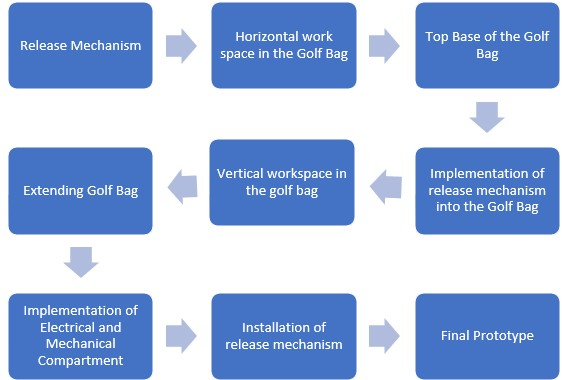
\includegraphics[width=0.8\textwidth]{Figure40.jpg}
            \captionof{figure}{Design Process}
            \label{fig:process}
        \end{center}
    \end{Figure}

\subsubsection{Design Process of Golf Bag Top Base }
Once the release mechanism as shown above had been
    decided, the golf bag provided by the client was dismantled to further
    understand its infrastructure. The original 
    segregation of the golf bag didn't reach the bottom of the golf bag Fig.
    (\ref{fig:cloth}). The segregation took place on the frame, a small part of
    the top part was segregated with cloth giving misconception that all  14
    golf clubs are well segregated. A segregation is
    essential to separate the release mechanism system and prevent the golf
    clubs from congestion with each other at the bottom of the golf bag. Therefore,    tube is implemented for each golf clubs so the golf clubs may not interact
    with each other. Different kinds of material for the tube had been explored such as plastic, acrylic and etc . PVC
    tube was chosen as it is cheap, accessible and lightweight. 
The inherited design is unsymmetrical and had
    inconsistent spacing, as shown in Fig. (\ref{fig:top}), for all the 14
    holes. Removing the inherited design will provide more freedom and
    potential to fully utilise the available space of the golf bag. Dimension was obtained by
scanning the top frame using a scanning machine. as shown in
     Fig. (\ref{fig:scan}). It is an innovative and efficient method to
    extract accurate data from irregular object due to its non-linear curvature.
    
    \begin{Figure}
        \begin{center}
            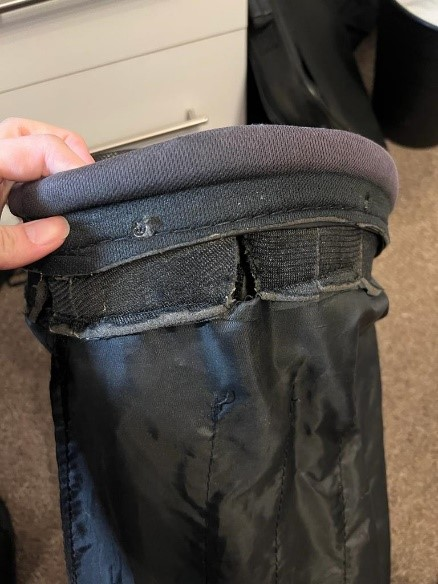
\includegraphics[width=0.3\textwidth]{Figure3.jpg}
            \captionof{figure}{Inherited Top Base Side View}
            \label{fig:cloth}
        \end{center}
    \end{Figure}
    
    \begin{Figure}
        \begin{center}
            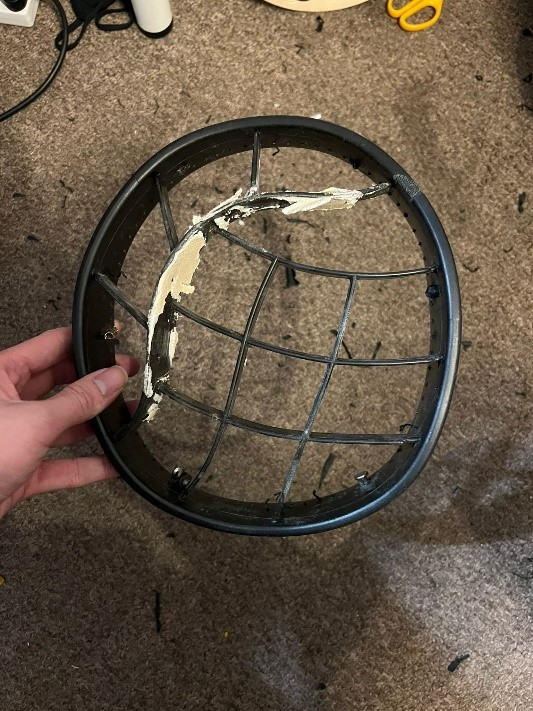
\includegraphics[width=0.3\textwidth]{Figure2.jpg}
            \captionof{figure}{Inherited Top Base Frame}
            \label{fig:top}
        \end{center}
    \end{Figure}
    
       From the scanned model in Fig. ( \ref{fig:CAD}), the area of the top part was calculated. With a fill factor of 80\%, it is feasible for each tube to have a
    maximum of 57mm outer diameter. Considering the average golf club handle to be 28mm, the tube 
    with 42mm outer diameter and 38mm inner diameter is the best options as it provides ease of
    placing the golf clubs into the tube. Using the given dimension, design had
    been made for the top base of the golf bag.
    
    The design of the bag will follow along the PVC tube.
. Each tube had its own name as specified
    golf clubs will be placed in them. By doing this, the machine learning will
    release the mechanism of the specified club to the golfer based on its
    decision with the acquired data from the golfer. 
        \begin{Figure}
        \begin{center}
            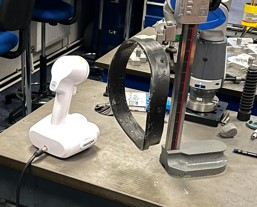
\includegraphics[width=0.5\textwidth]{Figure15.jpg}
            \captionof{figure}{Scan Machine}
            \label{fig:scan}
        \end{center}
    \end{Figure}
    
    
        \begin{Figure}
        \begin{center}
            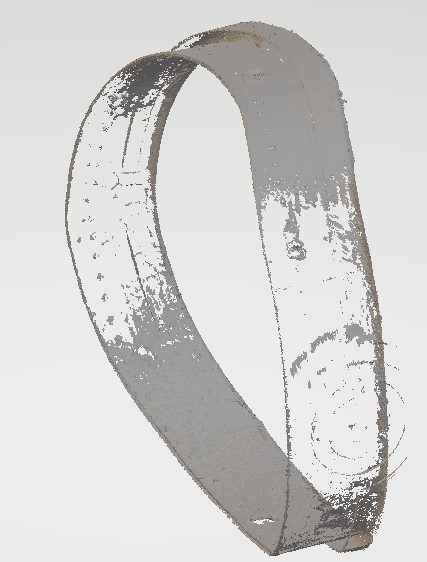
\includegraphics[width=0.3\textwidth]{Figure.jpg}
            \captionof{figure}{Result of 3D scan on caddy top}
            \label{fig:CAD}
        \end{center}
    \end{Figure}
    \subsubsection{Golf Bag innovation}
    The golf bag is another of our innovative creations as a fully-functioning
    golf bag with extremely low cost was produces. Low cost is achieved by reusing recycled
    items and using basic resources such as sheet metal, plywood and acrylic.
    Metal are used to extend the golf bag as it is flexible and cheap. . Plywood
    is used as the support for the release mechanism while acrylic is used for
    the new top base design of the golf bag. The golf bag functionality is well
    designed and is able to fulfil the design requirements.

    
    \subsubsection{Golf Bag Infrastructure}
      The whole bag had 3 different parts, the top base of the golf bag, the
    mechanical compartment and the electrical compartment as shown in Fig.
    (\ref{fig:golfbag}). The top base of the golf bag act as a support and
    segregation compartment for the golf clubs. The mechanical compartment
    consists of the motor compartment and the release mechanism. The motor is
    placed between two supports to ensure the motor is kept in place during
    operation. The release mechanism is above the motor compartment. It has a
    support base to ensure the tube and the release mechanism stays aligned. All
    the electronics and the cabling are placed in the electrical compartment to provide easy access for the future maintenance

    
    
    \begin{Figure}
        \begin{center}
            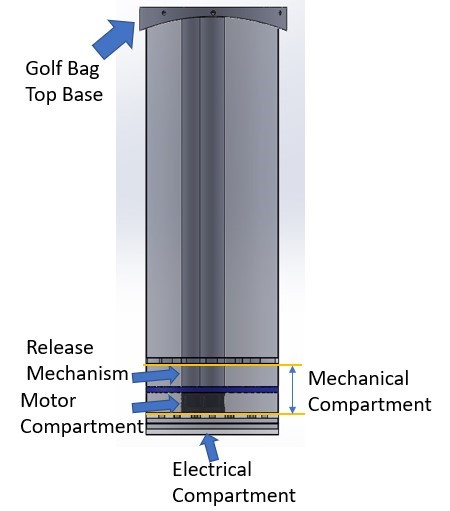
\includegraphics[width=0.8\textwidth]{Figure16.jpg}
            \captionof{figure}{Infrastructure of Golf Bag}
            \label{fig:golfbag}
        \end{center}
    \end{Figure}
    
    
    
    \subsubsection{Top base of Golf Bag}
    Two design had been implemented for the top base of the golf bag as shown in Fig. (\ref{fig:change}). The top base of the golf bag had 2 possible manufacturing process that can be used.
      
Design 1 had been initially laser cut with plywood before sending
    for 3D printing. The tube fit the design and is well supported by it.
    Due to the limitation of the 3D printer size (250 x 210 x 210mm), the new
    design had a dimension of (255 x 230 x 41 mm). Therefore it was not feasible
to 3D print the entire design.
It is cost effective and efficient to reuse the original top base frame of the golf bag as it can save manufacturing cost and time. 
    
    Decision was made to have the new design installed on the old golf bag 
    top frame which is more innovative as the frame could be reused. By reusing the frame, new connection part of the top base and the golf bag are not required. It can save manufacturing cost and time. The new
    design is drawn on Solidworks with the scanned CAD model of the top base shown in 
     Fig. (\ref{fig:CAD}). The final design is laser cut with acrylic and
    mounted on the frame with epoxy. The final top base is sprayed with black
    spray to improve aesthetic.

    \begin{Figure}
        \begin{center}
            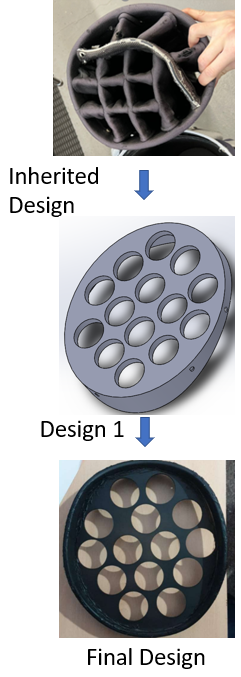
\includegraphics[width=0.4\textwidth]{Figure.png}
            \captionof{figure}{Design Process of Top Base}
            \label{fig:change}
        \end{center}
    \end{Figure}

    
    
    \subsubsection{Extension of Golf Bag}
    The golf bag is extended to fit the release mechanism. The release mechanism
    contributes an extra 138mm vertical height of the golf bag. The placing of the
    release mechanism is crucial as it may affect the overall performance. Due
    to the additional vertical height, the golf bag is extended to compensate
    the height from the release mechanism. Without the extension, the released
    golf clubs may injure the user since the golf clubs are released at a
    direction toward the user. The bag was extended using rolled metal
    sheet. Calculations were made for the circumference of the metal sheet.
    The metal sheet is spot welded to make a cylinder. The golf bag is
    extended by 150mm. 100mm are for the release mechanism, 38mm for the motor
    and 12mm for the electrical compartment.
    
    \subsubsection{Mechanical Compartment}
    The mechanical compartment consists of the mechanism and the stepper motor.
    As shown in Figure \ref{fig:SIDE} and \ref{fig:TOP}, the mechanism are
    installed on top of the stepper motor. The stepper motor is placed on the
    electrical top base. A motor base had been added to secure the motor between
    the motor base and the electrical base. The release mechanism is mounted on
    the motor base to ensure the mechanism stays stationary in the bag. The
    support base provides support to the PVC tubes and ensures the release
    mechanisms remained vertical.

    
    \begin{Figure}
        \begin{center}
            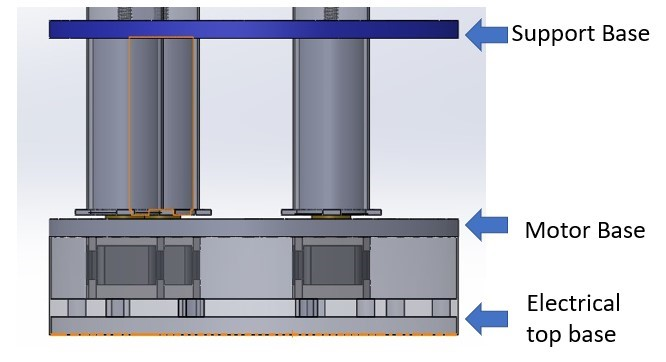
\includegraphics[width=\textwidth]{Figure6.jpg}
            \captionof{figure}{Side view of Mechanical Compartment}
            \label{fig:SIDE}
        \end{center}
    \end{Figure}
    
    \begin{Figure}
        \begin{center}
            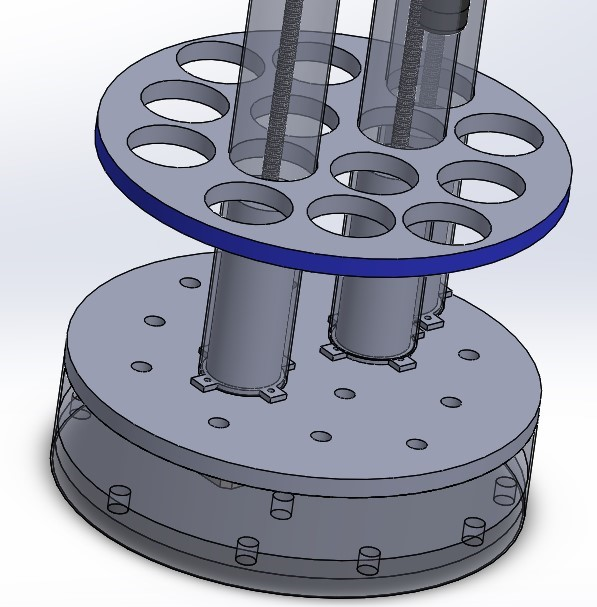
\includegraphics[width=0.5\textwidth]{Figure7.jpg}
            \captionof{figure}{Top view of Mechanical Compartment}
            \label{fig:TOP}
        \end{center}
    \end{Figure}
    
    \subsubsection{Electrical Compartment}
    The Electrical Compartment consist of a wooden laser cut top base and the
    original golf bag bottom base. The wooden laser cut base had 14 small holes
    on it as shown in Fig. (\ref{fig:ELECBASE}). The main function of the holes
    is to allow the electrical cable from the mechanical compartment to connect
    the electrical components.
    
    \begin{Figure}
        \begin{center}
            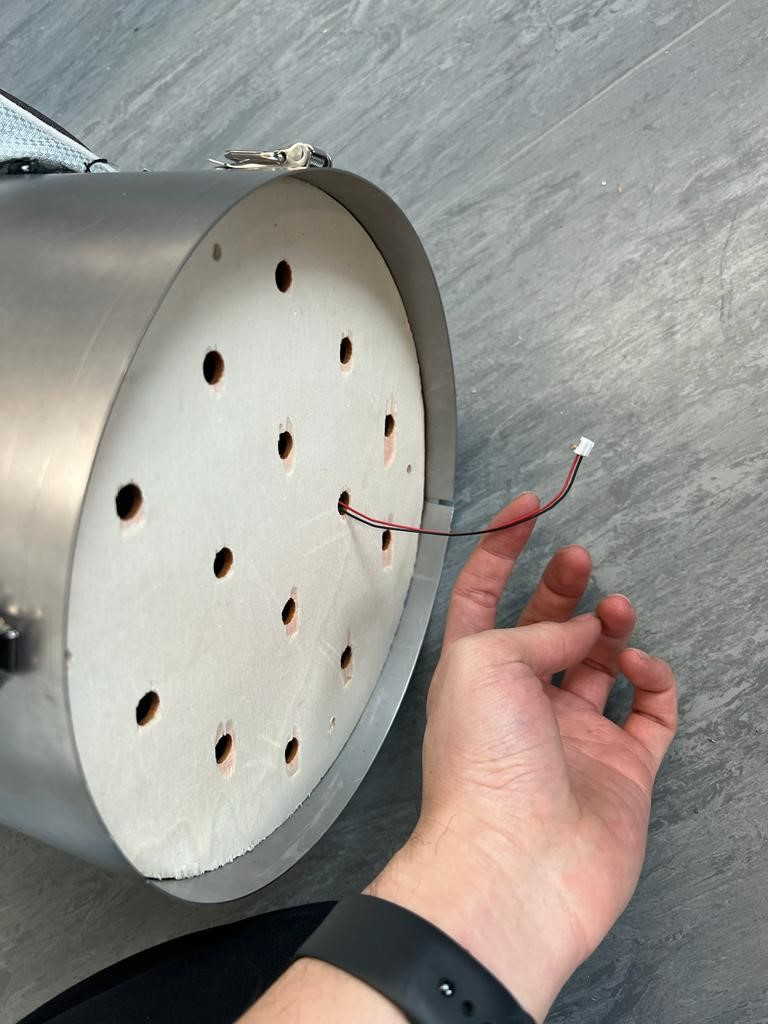
\includegraphics[width=0.6\textwidth]{Figure8.jpg}
            \captionof{figure}{Electrical Top Base}
            \label{fig:ELECBASE}
        \end{center}
    \end{Figure}
    
    
    
    \begin{Figure}
        \begin{center}
            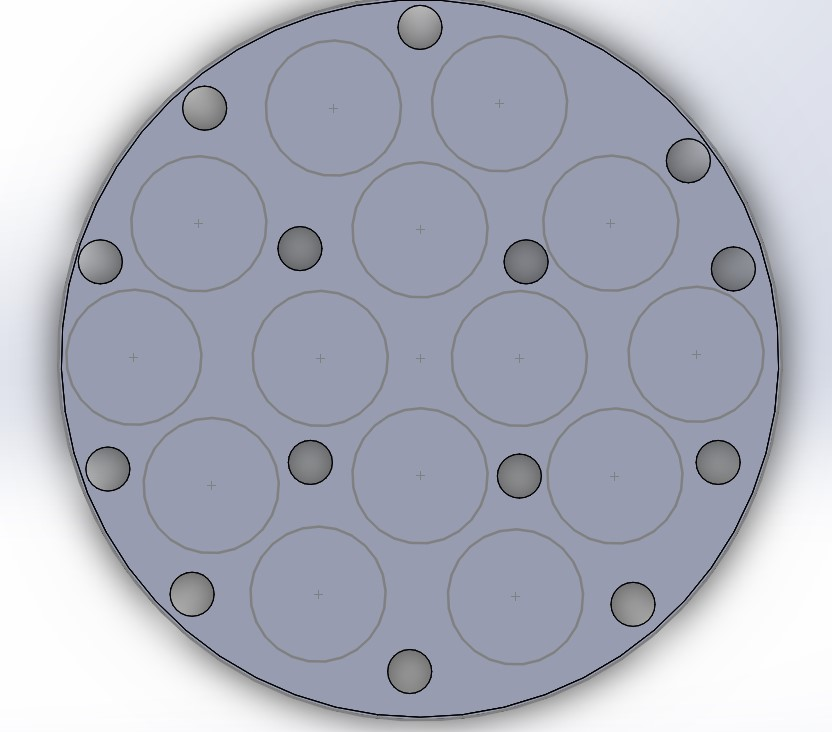
\includegraphics[width=0.5\textwidth]{Figure9.jpg}
            \captionof{figure}{Electrical Top Base CAD}
            \label{fig:ELEC}
        \end{center}
    \end{Figure}

    The location of the holes, shown in Fig. (\ref{fig:ELEC}), are placed beside the
    mechanical component to ensure none of the mechanical
    component will obstruct the hole. The electrical compartment consists of the
    cabling from the motor and a main cable which connects to the caddy. All the
    electronics are placed in the electrical compartment for ease of water
    proofing and to ensure the cabling do not disturb the mechanical system. 
    
    \subsubsection{Installation of release mechanism on golf bag }
    The support base was first mounted on the golf bag with a bracket. Once the
    extension of the golf bag are complete, the release mechanisms are installed
    on the motor base and mounted on the circular metal sheet with another
    bracket. The release mechanisms are installed into the PVC tube and the
    electrical top base are mounted below the stepper motor using a bracket.
    Finally, the inherited bottom base cover is placed below the circular
    metal sheet. Toggle latches are installed on both the circular metal sheet
    and the bottom cover to achieve easy accessible for the user. The process is
    shown in Figure \ref{fig:installation}.
    \begin{Figure}
        \begin{center}
            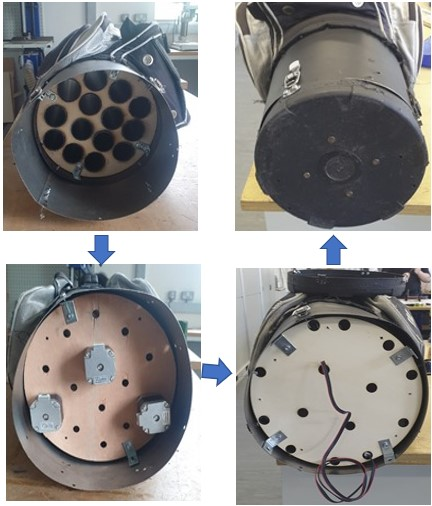
\includegraphics[width=0.6\textwidth]{Figure30.jpg}
            \captionof{figure}{Release Mechanism installation process in golf bag}
            \label{fig:installation}
        \end{center}
    \end{Figure}

    \subsection{LCD screen casing}
    In this project, a LCD screen is implemented which will have a GUI for data
    representation. A LCD screen casing was designed to protect the it from environmental damage such as rainwater and physical debris
    damage. Several possible location of mounting the LCD screen on the caddy are analyzed.
    The best location of mounting the LCD screen on the caddy will be
    below the caddy handle as it can be easily viewed by the user nearby
    the caddy. The location does not affect the folding operation of the caddy,
    as shown in Fig. (\ref{fig:holder}), as it utilized the abundant space of
    the AGC. 
 
    
    A 1 m electrical ribbon was used to connect the LCD screen with the
    Raspberry Pi located on the electrical housing of the caddy. The electrical
    ribbon is wrapped in heat shrink to provide protection and water
    resistance. The ribbon travels from the electrical housing of the AGC to
    the LCD screen through the AGC inner tube pathway as demonstrated in
     Fig. (\ref{fig:ribbon}).


    \begin{Figure}
        \begin{center}
            \includegraphics[width=0.8\textwidth]{Figure33.jpg}
            \captionof{figure}{HDMI ribbon path through AGC}
            \label{fig:ribbon}
        \end{center}
    \end{Figure}
    
    \subsubsection{Screen Holder}
        As shown in Fig. (\ref{fig:bottom}), the screen holder is mounted on the back of the bottom casing. The screen holder is designed to allow the LCD
    screen to sit firmly on the screen holder. A
    cylindrical metal rod Fig. (\ref{fig:rod}) was added in between the
    screen holder to ensure the screen holder does rotate more than 90 degrees.

    
    \begin{Figure}
        \begin{center}
            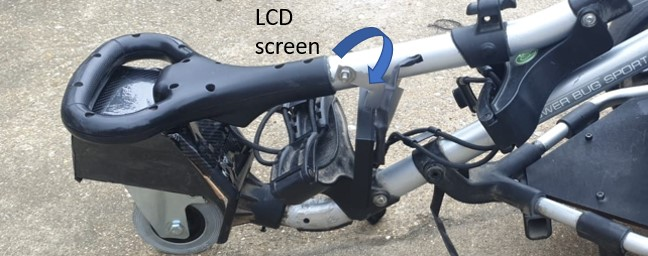
\includegraphics[width=\textwidth]{Figure39.jpg}
            \captionof{figure}{AGC folded with screen}
            \label{fig:holder}
        \end{center}
    \end{Figure}
    
    \begin{Figure}
        \begin{center}
            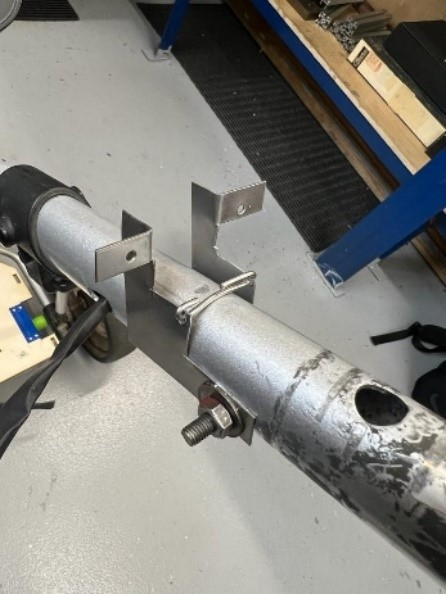
\includegraphics[width=0.6\textwidth]{Figure31.jpg}
            \captionof{figure}{Screen holder with metal rod support}
            \label{fig:rod}
        \end{center}
    \end{Figure}
    
    \subsubsection{Friction Hinge}
    The screen can be fold and unfolded by 90 degrees using the friction hinge
    concept shown in Figs. (\ref{fig:unfold} \ref{fig:fold}). The screen
    holder is designed to operate along with the friction hinge operation. The
    friction hinge relies on the friction provided from the nuts and bolts. By
    providing sufficient friction, the screen could be fixed and folded easily.
    
    \begin{Figure}
        \begin{center}
            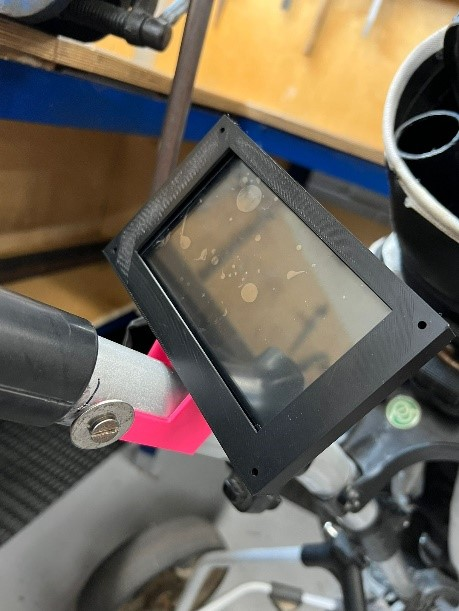
\includegraphics[width=0.5\textwidth]{Figure17.jpg}
            \captionof{figure}{Unfold LCD screen}
            \label{fig:unfold}
        \end{center}
    \end{Figure}
    
    \begin{Figure}
        \begin{center}
            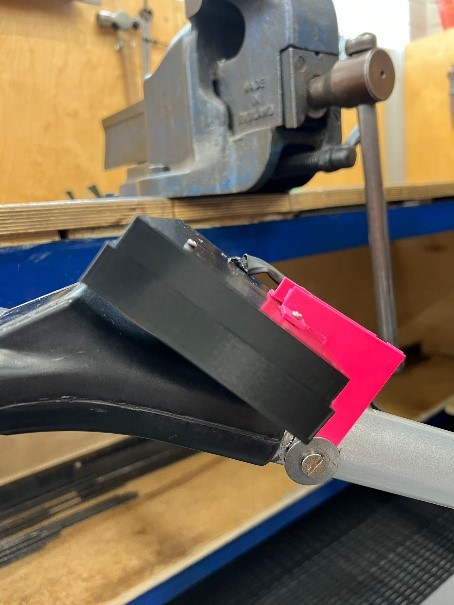
\includegraphics[width=0.6\textwidth]{Figure18.jpg}
            \captionof{figure}{Folded LCD screen}
            \label{fig:fold}
        \end{center}
    \end{Figure}
    
    
    \subsubsection{Bottom casing}
    The bottom casing is designed according to the needs of installation and the
    electrical requirements. The LCD screen fits the bottom casing perfectly as shown in
    Fig. (\ref{fig:LCD}). From Fig. (\ref{fig:bottom}), there is a slot to allow
    connection for the electrical ribbon from the screen to the AGC. Bolts are
    used to screw directly on the LCD screen through hole 1 and hole 2. While
    the bolts on hole 3 and 4 will go through the screen holder before screwing
    on the LCD screen. Therefore, the bottom case will mount firmly to the
    screen holder.
    
    \begin{Figure}
        \begin{center}
            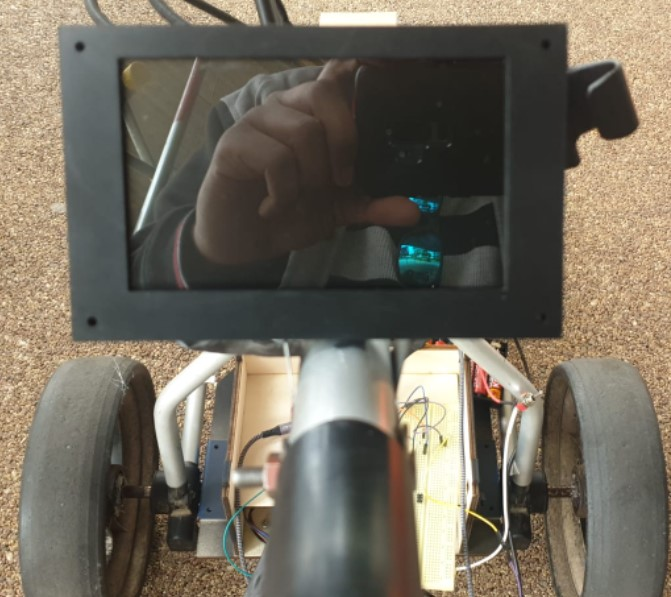
\includegraphics[width=0.8\textwidth]{Figure32.jpg}
            \captionof{figure}{Front view of LCD screen fit in casing}
            \label{fig:LCD}
        \end{center}
    \end{Figure}
    
    
    \begin{Figure}
        \begin{center}
            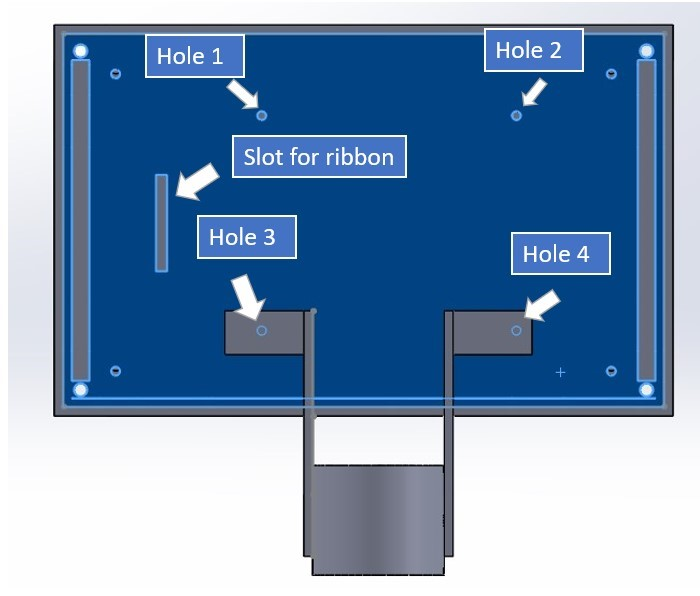
\includegraphics[width=0.8\textwidth]{Figure11.jpg}
            \captionof{figure}{Back view of Bottom casing}
            \label{fig:bottom}
        \end{center}
    \end{Figure}
    

    \subsubsection{Top casing}
    The top screen covers the bottom casing edges and the LCD screen to ensure
    no water flow to the internal screen casing. A screen protector is installed
    on the large empty slot of the top screen. The selected screen protector is
    made of tempered glass which doesn’t affect the touch screen functionality.
    The screen protector is glued on the casing and a layer of resin is added to
    prevent water intake. The screen protector provides the ability of using the
    LCD screen during rainy condition as it is well water-proofed. The top
    casing are mounted with the bottom casing with nuts and bolts through Hole
    C,D,E,F as shown in Fig. (\ref{fig:HOLE}) This ensures the entire casing
    does not drop from the screen holder during motion.
    
    \begin{Figure}
        \begin{center}
            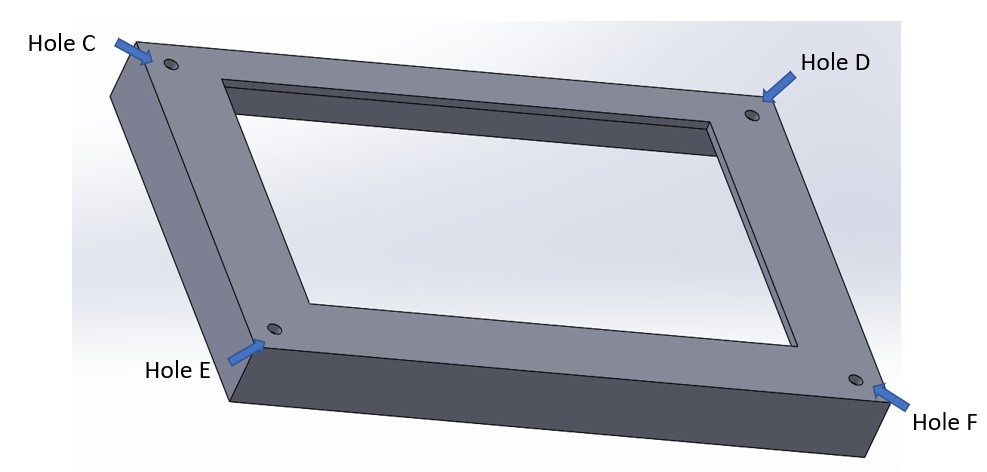
\includegraphics[width=0.8\textwidth]{Figure13.jpg}
            \captionof{figure}{Top Casing with holes}
            \label{fig:HOLE}
        \end{center}
    \end{Figure}
\end{multicols}

\newpage
\begin{multicols}{2}
    \subsection{Golf Cart Caddy Electrical Base}
    From the inherited golf caddy, there were close to no electrical systems
    since only the wheels were motorised. However, with the addition of all the
    newly added electrical systems from this project, an electrical base was
    required in order to house all the electrical circuits that were made. The
    list of components that will be in the electrical base are the EMG49 motors,
    MD49 driver, Raspberry Pi, GPS module, battery regulation circuit and
    release mechanism circuits.
    
    \subsubsection{Concept Design}
    After investigating the inherited golf caddy for possible locations that can
    be used for the electrical base, it was determined that the only
    feasible place was where the previous battery was located. After removing the
    previous motors and battery plate holder, the new allocated space was
    measured and built on SOLIDWORKS in order to model different possible design
    for the electrical base. Fig. (\ref{fig:base}) shows the available space
    from the caddy after the motors were removed.
    
    \begin{Figure}
        \begin{center}
            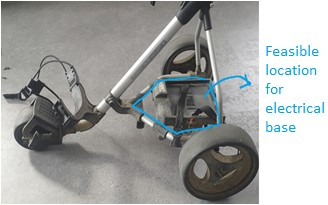
\includegraphics[width=0.8\textwidth]{Figure22.jpg}
            \captionof{figure}{Location for electrical base}
            \label{fig:base}
        \end{center}
    \end{Figure}
    
    Three possible designs were initially made on CAD and they are shown in
    Fig. (\ref{fig:box}).
    
    \begin{Figure}
        \begin{center}
            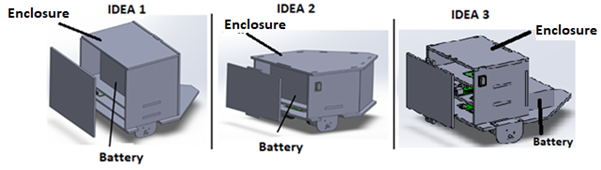
\includegraphics[width=1.0\textwidth]{Figure23.png}
            \captionof{figure}{Concept design for electrical base}
            \label{fig:box}
        \end{center}
    \end{Figure}
    
    
    Idea 3 was chosen as the best option since it allows for an easy access to
    the electrical components which is beneficial for maintenance and fault
    checking should any issues occur. It also allows the user to easily remove
    and charge the battery when required without interfering with any of the
    electrical circuits along the way and it provides a better airflow compared
    to being clustered in the enclosure compartment. It is also beneficial for the
    centre of mass of the AGC as the battery, which is the heaviest amongst
    the components on the electrical base, is as close as possible to the centre
    of the AGC. It allows for a more stable drive whilst minimising the chance
    of the AGC toppling over when going on a hill. The combined weight of all
    the components that will be in the base was determined to be about 7 kg.
    Based on this and the fact that this base is only being used for testing
    since this project is at the prototype stage, it was determined that 6 mm
    birch plywood was the best material of choice. It is cheap, easily
    accessible and can provide enough strength to hold all the components as
    well as being lightweight enough to not have an impact on the motors. Laser
    cutting was used as the manufacturing process for time saving and due to the
    possibility of employing box joints as well as mortise and tenon joints in
    order to easily assemble the design. The joints were further reinforced
    using adhesive for added reassurance of the structural integrity of
    the design.
    
    
\subsubsection{Final Design}
Fig. (\ref{fig:final}) shows a detailed assembly with the component of the base
and Fig. (\ref{fig:blackcaddy}) shows the implemented base on the caddy

\begin{Figure}
    \begin{center}
        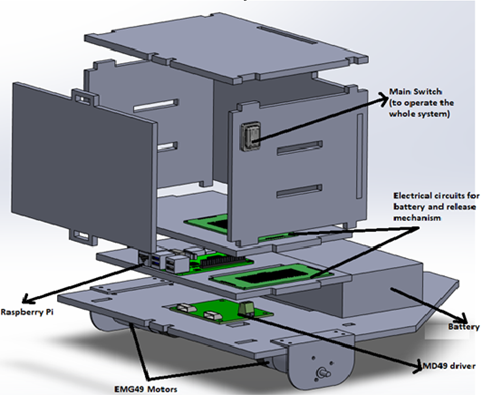
\includegraphics[width=\textwidth]{basefinal.png}
        \captionof{figure}{Assembly of proposed electrical base design}
        \label{fig:final}
    \end{center}
\end{Figure}

\begin{Figure}
    \begin{center}
        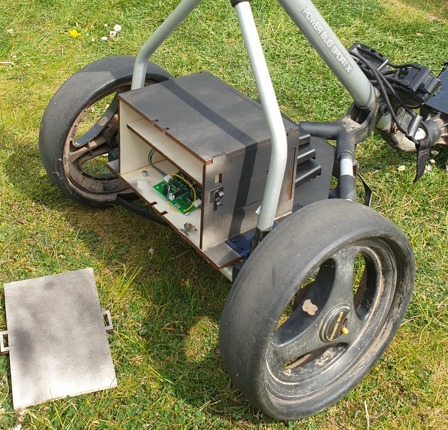
\includegraphics[width=0.6\textwidth]{Figure37.jpg}
        \captionof{figure}{Implemented electrical base on caddy}
        \label{fig:blackcaddy}
    \end{center}
\end{Figure}
    
\subsection{Powertrain and Wheels}
The powertrain on the inherited golf AGC consisted of a motor which was
powering the rear wheels on a single axle. It allowed the caddy to be
remotely controlled which was used to assist the user in pushing the caddy
around. However, a user input was still required in order to navigate the
caddy, for example when changing direction, since the front wheels were
attached in such a way that would only allow forward and backward drive.
Fig. (\ref{fig:train}) shows the drivetrain of the inherited caddy.

Due to the introduction of the autonomous tracking system and release
mechanism, new motors are required in order to propel the AGC with the
extra added weight. This powertrain required some changes to be made since
it was not designed for autonomous driving.

\subsubsection{Design Requirement for Powertrain}
Two important design changes were identified. Since the AGC will have to
make turns when required during the autonomous tracking, a speed
differential between each of the rear wheel is required. Therefore, two
separate motors are needed to control each rear wheel individually.
Furthermore, a ball castor type support should be added at the front of the
AGC in order to facilitate the turning action of the AGC as well as
providing the ability for the AGC to have its own centre of rotation. 
    

\begin{Figure}
    \begin{center}
        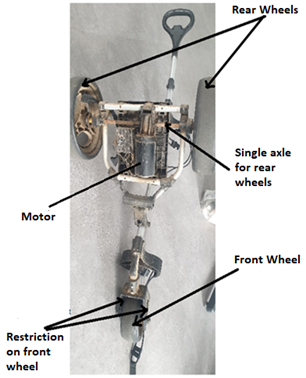
\includegraphics[width=\textwidth]{Picture2.PNG}
        \captionof{figure}{Inherited Caddy Powertrain}
        \label{fig:train}
    \end{center}
\end{Figure}
\newpage
\subsubsection{Rear Wheel}
In order to be cost effective and time efficient instead of manufacturing or
buying a wheel from a third party seller, the previous rear wheels were
used. However, these wheels were not compatible to be attached directly to
the new motors since it required a locking mechnaism that is located on the
previous axle. Therefore, this axle was cut down at two separate locations
in order to retain this locking mechanism as well as a bracket that is used
to securely connect it to the main frame of the caddy. Fig. (\ref{fig:rear})
shows the locations that were determined to be the optimum cut off points.

\begin{Figure}
    \begin{center}
        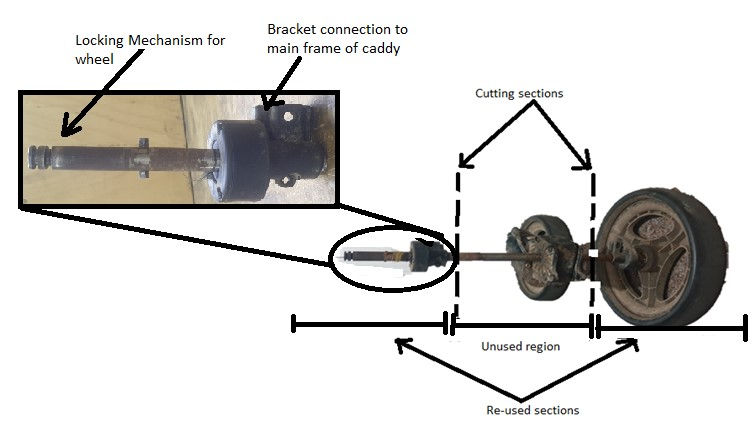
\includegraphics[width=\textwidth]{Figure26.jpg}
        \captionof{figure}{Rear axle from inherited golf caddy}
        \label{fig:rear}
    \end{center}
\end{Figure}

Considering the space available, where the wheels need to be mounted, and
the dimensions of the motors to be used, the connection between the shaft of
the motor and the axle needs to be close type and secure connection. Since
welding was not feasible due to the contact surface being too small between
the motor shaft and the axle, adhesive was used. In order to have more
contact surface when applying the adhesive, the motor shafts were immersed
inside the axles where it allows for more robust coupling. Fig.
(\ref{fig:auto}) shows the rear wheels attached to the motors and mounted on
the base plate of the electrical base.

\begin{Figure}
    \begin{center}
        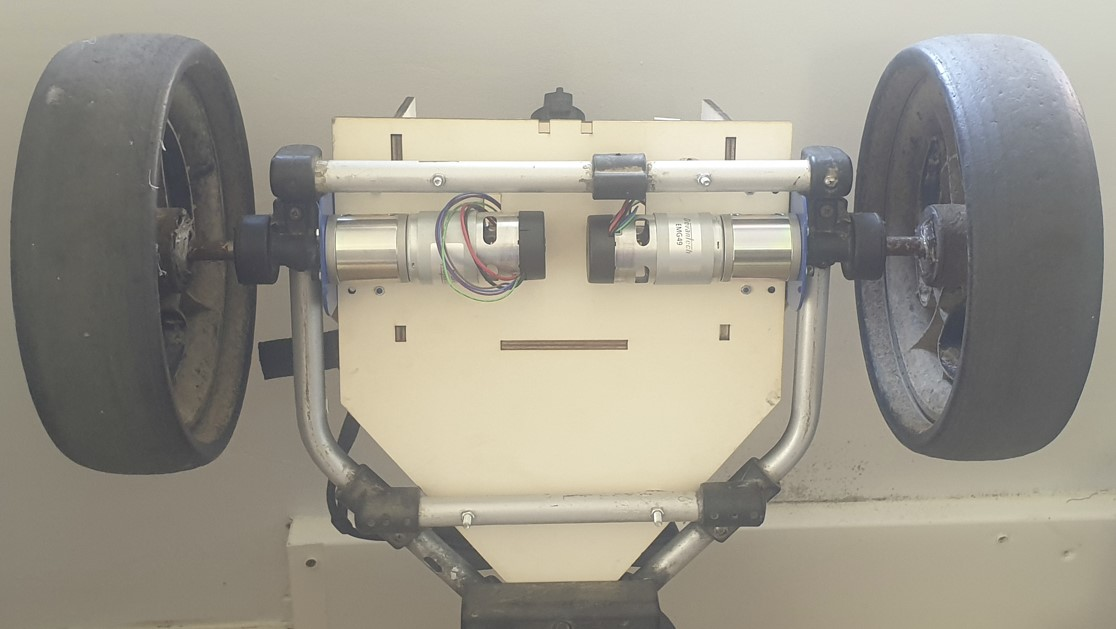
\includegraphics[width=\textwidth]{Figure27.jpg}
        \captionof{figure}{Autonomous driving compatible powertrain}
        \label{fig:auto}
    \end{center}
\end{Figure}


\subsubsection{Front Wheel}
The front wheel was decided that it will be incompatible to be used for
autonomuos driving and therefore a swivel castor wheel was chosen as its best
replacement. After removing the intial front wheel and its restrictions, the
mounting space was at an incline fo 45 degrees. Since a flat surface is required
to mount the swivel castor wheel, a piece of wood was cut to the appropriate
dimension, in order to fill the gap. The wooden piece dimension also took
into account the range of rotation of the wheel. Fig. (\ref{fig:castor}) shows
the process for mounting the swviel castor wheel on the caddy. 

\begin{Figure}
    \begin{center}
        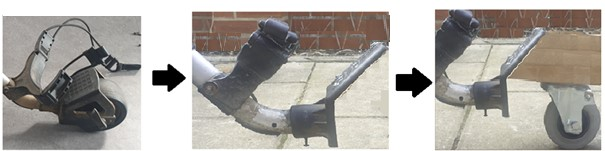
\includegraphics[width=\textwidth]{Figure28.jpg}
        \captionof{figure}{Swivel Castor Wheel installation process}
        \label{fig:castor}
    \end{center}
\end{Figure}
The wooden piece was later wrapped in vinyl for aesthetic purposes.

\newpage
\subsubsection{Wheel Assembly}
Fig. (\ref{fig:sprayed}) shows the wheels mounted on the golf AGC. 

\begin{figure}[H]
    \begin{center}
        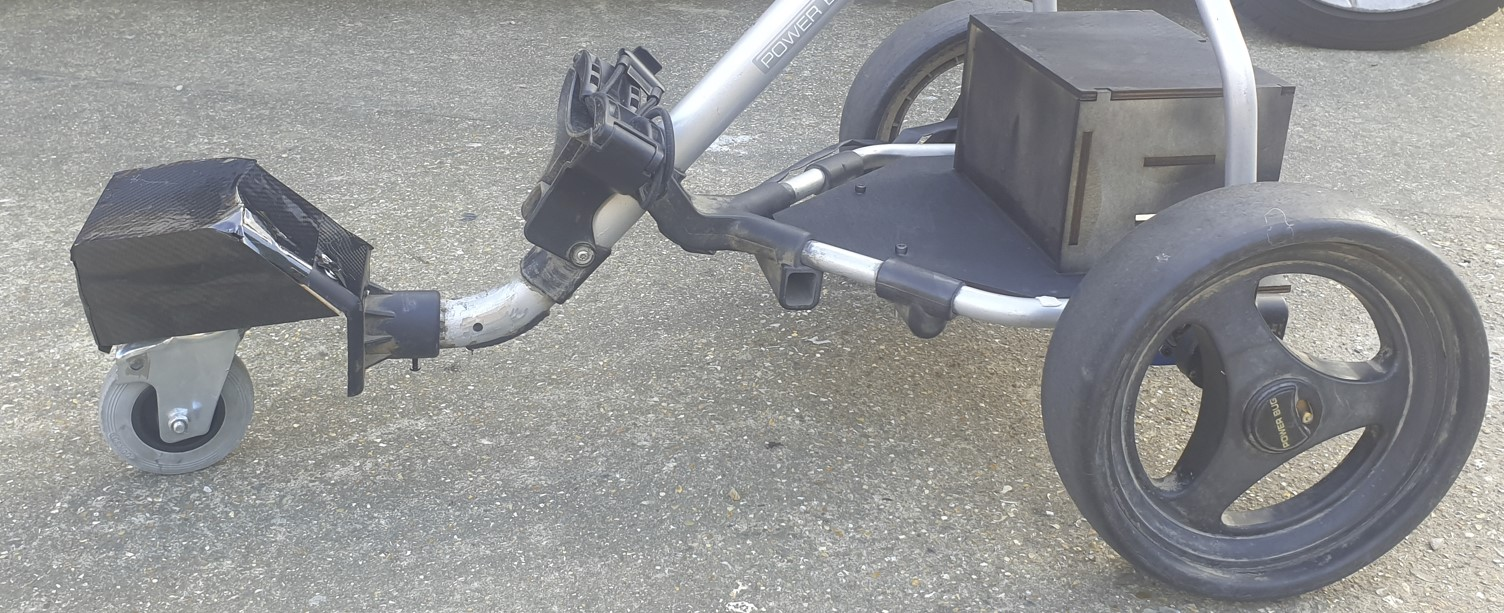
\includegraphics[width=0.5\textwidth]{Figure29.jpg}
        \captionof{figure}{Full Wheel installation process}
        \label{fig:sprayed}
    \end{center}
\end{figure}


\subsection{Further Improvement}

For the continuation of this project, to make it a commercially viable
product, the future team undertaking it should consider the following.

\subsubsection{Release Mechanism}
For the release mechanism, one of the key improvements that could be
implemented would be the use of gears for the mechanism as it can save up a
lot of weight instead of using one stepper motor per golf club. Other
materials such as acrylic, wood or stiffer steel should be explored in order
to be used as the guiding rails since the current one being used are
threaded rods of 2 mm diameter which can easily bend. This can cause issues
to the release mechanism’s elevating platform since it can get stuck at the
point where the bending of the guiding rails occurs. Currently, the way to
operate the release mechanism, requires the user to connect the cable from
the golf bag to the caddy’s electrical base. An improvement to that could be
to implement a circuit within the golf bag that can communicate with the
circuit on the golf AGC through WiFi or Bluetooth, thus reducing the
possibility of the connection being loose or faulty which would not allow the system
to work. It also benefits the user since they will not have to worry about
unintentionally pulling the circuit system inside the electrical base on the
caddy every time they remove the golf bag form the golf caddy. 

\subsubsection{Golf Bag}
The current golf bag is designed to be able to implement waterproofing. Due
to time constraint, the concept had not been implemented but could be done
easily with the current golf bag. Both mechanical and electrical Compartments
could be sealed with resin to prevent water entering the system. A water
sink could be implemented above the Mechanical Compartment. A tube could be
used to release the accumulated water from the water sink.

\subsubsection{Golf Caddy Infrastructure}
The golf caddy could be more futuristic if the AGC chasis could be redesigned.
Function of one button folding and unfolding could be achieved if the AGC is
well designed.

\subsubsection{Caddy's Electrical Base}
It might be better to explore further designs since the current base is too
tall and it does not allow the full closure of the AGC when the golf bag
is removed. The need for waterproofing the “box” compartment which contains
all the electrical circuits should be implemented in the design stage as one
of the key design requirements. The current way to close the base is just a
sliding type of closure and it could be improved by using hinges or some
other component that can make the base more compact with regards to the
waterproofing. In terms of material selection, it might be better to use
acrylic for a commercially viable product since it will look better
aesthetically. 

\subsubsection{Front Wheel}
In terms of the current connection of the swivel castor wheel, it might be
best to make changes to the main frame of the golf AGC instead of using
the piece of wood to make a flat surface. Moreover, the front wheel itself
should be considered to change since it might not provide enough grip to be
used on a golf course for a long period of time.
    
\end{multicols}


\newpage
\begin{multicols}{3}
\section{Software}
\label{software}
In this section all software required for the operating cycle of the AGC is
discussed. The AGC main computer is a Raspberry Pi 4 running a 64-bit Debian
port, the same for the Raspberry Pi used in the tracking pod. The GPS
navigation system requires high precision decimal storage to operate properly.
Data type \verb|float32| can store 23 significant bits, compared to data type
\verb|float64| which can store 52 significant
bits\cite{floating_point_goldberg}. The calulcations shown below in Fig.
(\ref{fig:float_calcs}) show the physical significance of which datatype is
chosen.
\begin{figure}[H]
    \begin{mdframed}
        Only $180^{\circ}$ need to be accounted for because sign bit is
        separate, so to represent $180^{\circ}$ the bits required is:
        \begin{center}
            \begin{equation*}
                \log_2{180} \approx 7.49185 bits
            \end{equation*}
        \end{center}
        This leaves the $n - 7.49185$ significant bits left for sub degree
        representation, the physical precision in meters can be derived from
        each data type of a longitude value at the equator can be calculated as
        shown in the equations below.\newline
        \begin{center}
            \begin{minipage}{0.45\textwidth}
                \begin{mdframed}
                    For \verb|float32| $n=23$:
                    \begin{center}
                        \begin{equation*}
                            \frac{\frac{R_e \cdot \pi}{180}}{2^{\left(52 - \log_2{180}\right)}} \approx 2.386m
                            \label{eq}
                        \end{equation*}
                    \end{center}
                \end{mdframed}
                \end{minipage}
                \begin{minipage}{0.45\textwidth}
                    \begin{mdframed}
                For \verb|float64| $n=52$:
                \begin{center}
                    \begin{equation*}
                        \frac{\frac{R_e \cdot \pi}{180}}{2^{\left(52 - \log_2{180}\right)}} \approx 4.44nm
                    \end{equation*}
                \end{center}
            \end{mdframed}
            \end{minipage}
        \end{center}
        \center The radius of Earth. $R_e$, value used was $6371000m$. 
    \end{mdframed} 
    \captionof{figure}{Calculations showing physics precision of single vs
    double precision floats}
    \label{fig:float_calcs}
\end{figure}
The $180^{\circ}$ is normalised to a power of two so it is possible to use the
non integer value of bits in the calculation for physical precision. Were this
normalisation not performed then $7.4918\rightarrow8$ full bits are required to
represent the degrees and the final precision is slightly less for each
datatype. To ensure this calculated precision is representative of our system
all GPS coordinates are normalised to a power of two. It can be seen from the
calculations that a significantly higher precision is achieved using double
precision floating point data type to store GPS values. The precision yielded by
the double precision floating point is unnecessary, however the precision of the
single precision floating point is too low as our GPS module is capable of
providing more accurate GPS measurements as discussed in section
\ref{electronics}. Therefore double precision floating point datatypes will be
used to store GPS data, which requires use of a 64-bit compatible operating
system which is why the 64-bit Debian port was chosen. The higher precision
achieved comes at the cost of slightly higher compte time for calculations,
however as most of the algorithms onboard operate only on small amounts of data,
this effect is unnoticable when operating the AGC.

\subsection{Control Software}
\label{control_software}
This section discusses the software used to make the AGC follow the golfer. All
of the control software apart from the elctronics specific code, such as motor
controller communication, was written first in the OpenGL simulator environment
that was built throughout the year. Building and using a simulator allowed
writing and testing of all the control software / algorithms that would be
required to make the AGC follow the golfer as intended while avoiding hazard
regions. All control software can be found
\href{https://github.com/GDP-50/Onboard-RasPi}{here on GitHub.}

All of the control software tested in the simulator was written in C as this was
easiest to use with OpenGL, however it was decided to change to PyQt5 for designing
the onboard GUI. As the ACG software was now to be written in Python the control
algorithms were re-written in Python, however upon testing it was found that
their performance was significantly slower than the C implementations. This is
most likely a large amount of array passing and manipulations are required,
which is significantly slower in Python where function arguments are passed as
object reference instead of pointers in C. Therefore the original C control
algorithms were compiled as a dynamic link library (DLL) and the Python ``C
Types'' library was used to load the DLL and create Python wrappers for the
control algorithms. This significantly improved the performance as all of the
resource intensive calculations were now performed with a compiled C program.

\begin{Figure}
    \begin{center}
        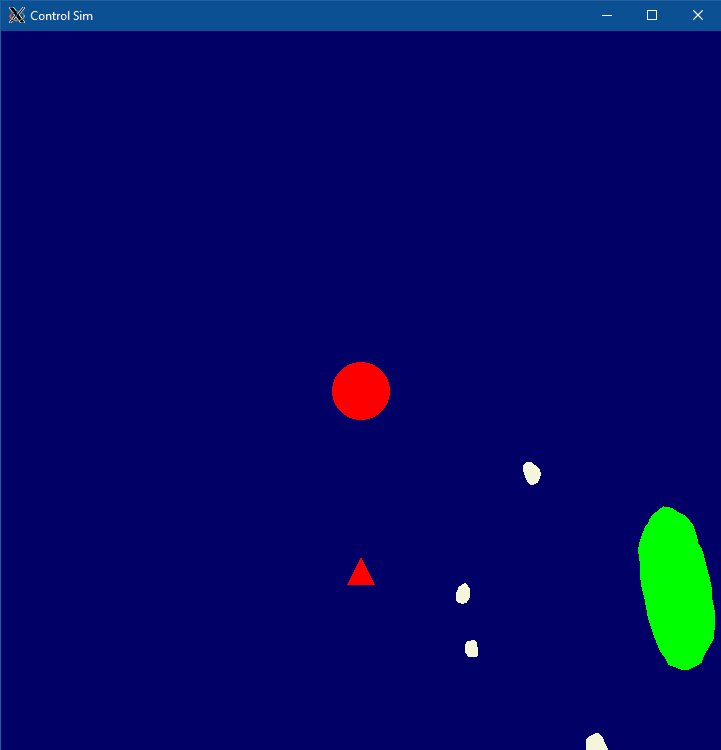
\includegraphics[width=\textwidth]{simulator.png}
    \end{center}
    \captionof{figure}{Simulator used for algorithm testing}
    \label{fig:simulator}
\end{Figure}
\vfill\null
\columnbreak
The main control loop that determines the AGC's behaviour is shown in Fig.
(\ref{fig:control_loop}).
\begin{Figure}
\begin{mdframed}
    \begin{center}
        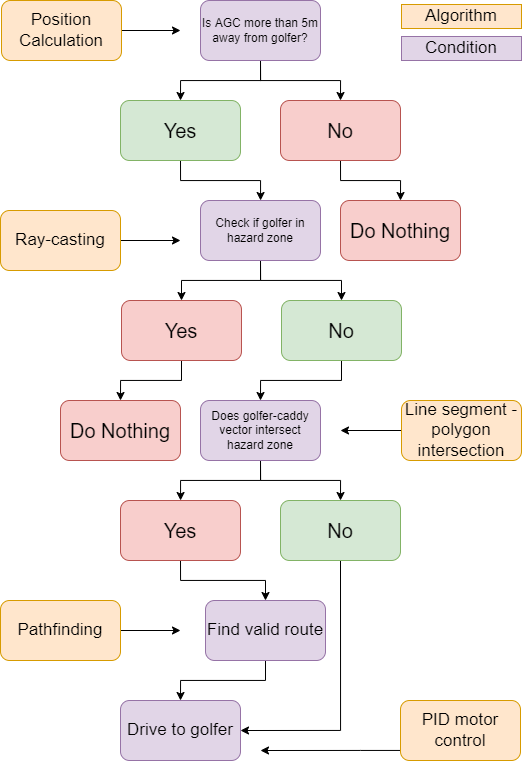
\includegraphics[width=0.9\textwidth]{control_loop.png}
    \end{center}
\end{mdframed}
\captionof{figure}{Main AGC control loop}
\label{fig:control_loop}
\end{Figure}
\subsubsection{Design and Test Process}
All software used for controlling the AGC was tested on the OpenGL simulator
built. This allowed for good visualisation and analysis of the algorithms'
performance. Only the pathfinding algorithm was not tested on the simulator to
prevent wasting time animating it; visual output using Matplotlib was more
efficient.

\subsubsection{Map Processing}
As discussed in the introduction to section \ref{software}, all GPS coordinates
are normalised to a power of two. Also, the hazard zones are ``padded''  by a
safety factor of two meters, preventing innacurate GPS readings or hazard zone
coordinates resulting in the AGC entering a hazard zone. The hazard zones are
``padded'' by calculating the coordinates of centroid of the polygon, then
extending the vector from the centroid to each perimeter point by two meters.
The centroid of a polygon can be calculated from the coordinates of it's
perimeter points as shown in Eqs. (\ref{eq:cx} and \ref{eq:cy}).
\begin{center}
    \begin{equation*}
        A=\frac{1}{2}\sum_{i=0}^{n-1}\left( x_i y_{i+1} - x_{i+1} y_i\right)
    \end{equation*}
\end{center}
\begin{center}
    \begin{equation}
        C_x=\frac{1}{6A}\sum_{i=0}^{n-1} (x_i + x_{i+1}) (x_i y_{i+1} - x_{i+1} y_i)
        \label{eq:cx}
    \end{equation}
\end{center}
\begin{center}
    \begin{equation}
        C_y=\frac{1}{6A}\sum_{i=0}^{n-1} (y_i + y_{i+1}) (x_i y_{i+1} - x_{i+1} y_i)
        \label{eq:cy}
    \end{equation}
\end{center}
\subsubsection{Ray Casting}
The ray casting algorithm is used to determine whether a point falls within a
polygon. The algorithm can only accept polygons with straight edges; our
polygons are represented by a series of GPS points along their perimeter, and so
our polygons are defined by a series of small straight edges. The concept of
this algorithm is that given a point you wish to test, if you cast a ray from
the point in one direction to infinity, the number of intersections the ray has
with the polygon in question indicates whether the point falls in the polygon or
not. If an even number of intersections are found, then the point lies outside
the polygon, and if an odd number of intersections are found the point lies
within the polygon. Zero intersections means the point lies outside the polygon.
A visual of this concept can be seen below in Fig. (\ref{fig:raycasting}).
\begin{figure}[H]
    \begin{mdframed}
        \begin{center}
            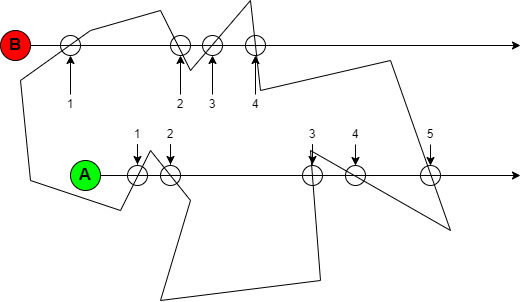
\includegraphics[width=0.95\textwidth]{raycasting.png}
        \end{center}
    \end{mdframed}
    \captionof{figure}{Raycasting Example}
    \label{fig:raycasting}
\end{figure}

The figure shows two points which are to be tested to determine if they lie
within the polygon. Casting the ray to the right, towards $x\rightarrow\inf$ in
our implementation, the intersections each ray has with the polygon are counted.
Point A has five intersections and so lies inside the polygon, point B has four
intersections and lies outside the polygon. 

There are additional considerations in our implementation to accout for the ray
intersecting a vertex or for the ray being collinear with a polygon edge. If a
vertex is encountered on the ray then two intersections are counted, one for each edge
forming the vertex, and the result is not affected. If the ray is collinear with
a polygon edge then only a single intersection is counted, but the ray will
undoubtedly also intersect at least one of the vertices on the collinear edge
which will be appropriately accounted for. The algorithm has been tested and
does not fail in either of these cases.

\subsubsection{Segment Polygon Intersection}
Before the AGC starts moving towards any target destination, it first checks
that it's intended translation vector joining it's location to the target
location does not pass through any hazard zones. It does this by checking that
it's intended translation vector doesn't intersect any edges of polygons. The
diagram shown below in Fig. (\ref{fig:segment_intersection}) depicts two finite
length line segments intersecting.
\begin{figure}[H]
    \begin{mdframed}
        \begin{center}
            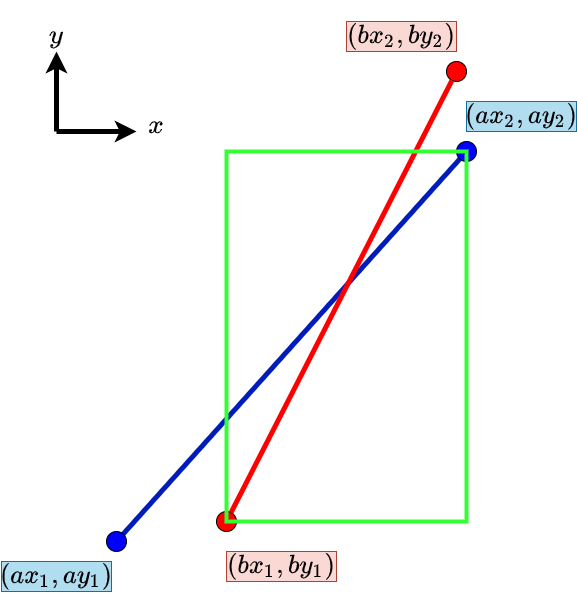
\includegraphics[width=0.95\textwidth]{segment_intersection.png}
        \end{center}
    \end{mdframed}
    \captionof{figure}{Line Segment Intersection Diagram}
    \label{fig:segment_intersection}
\end{figure}
 
The edges of polygons are defined only by the positions of two vertices, as is
the AGC intended translation vector. To calculate where the intersection point
of these two line segments are a mathematical equation for a line must be
constructed for each segment as shown in Eqs. (\ref{eq:line_a} and
\ref{eq:line_b}) respectively, then these equations can be solved simultaneously
to determine the location of the intersection as shown in Fig.
(\ref{fig:segment_calculations}).

After the intersection point is calculated it is ensured that the intersection point
falls within the smallest rectangle bounded by one point from the first and
second coordinates of either segment. This is done because the equation for a line
is infinite, and any lines with non equal gradient will intersect, but it is
only relevant if the intersection occurs between points the AGC intends to
travel. The bounding rectangle is demonstrated by the green rectangle in Fig.
(\ref{fig:segment_intersection}).

\begin{figure}[H]
    \begin{mdframed}
        \begin{center}
            \begin{equation}
                ay_1-y = \frac{ay_2 - ay_1}{ax_2 - ax_1} \times (x - ax_1)
                \label{eq:line_a}
            \end{equation}
            \begin{equation}
                by_1-y = \frac{by_2 - by_1}{bx_2 - bx_1} \times (x - bx_1)
                \label{eq:line_b}
            \end{equation}
        \end{center}
    In our implementation, before this system is solved, it is checked for if
    the lines have equal gradient, and if they are collinear or not. If they
    have equal graident, defined by:
    \begin{center}
        \begin{equation*}
            \frac{ay_2 - ay_1}{ax_2 - ax_1} = \frac{by_2 - by_1}{bx_2 - bx_1}
        \end{equation*}
    \end{center}
    The condition for collinearity must be checked, defined by:
    \begin{center}
        \begin{equation*}
            (x - ax_1) = (x - bx_1)
        \end{equation*}
    \end{center}
    If they are collinear then they intersect, if the have equal gradient but
    are not collinear then they do not intersect. If one or both of the lines
    are vertical, $(y_1 = y_2)$ then the system is not solved as below but
    trivially using the $x$ position of the line.\vspace{0.5cm}
    \newline
    For simplification:
    \begin{center}
        \begin{equation*}
            m_a = \frac{ay_2 - ay_1}{ax_2 - ax_1} \hspace{1cm} m_b = \frac{by_2 - by_1}{bx_2 - bx_1}
        \end{equation*}
    \end{center}
    The system must be solved using Eqs. (\ref{eq:line_a} and
    \ref{eq:line_b}) to determine the point of intersection resulting in the $x$
    coordinate given by Eq. (\ref{eq:x}) and $y$ coordinate given by Eq.
    (\ref{eq:y}).
    \begin{center}
        \begin{equation}
            x = \frac{ax_{1} m_{a} - ay_{1} - bx_{1} m_{b} + by_{1}}{m_{a} - m_{b}}
            \label{eq:x}
        \end{equation}
        \begin{equation}
            y = \frac{ax_{1} m_{a} m_{b} - ay_{1} m_{b} - bx_{1} m_{a} m_{b} + by_{1} m_{a}}{m_{a} - m_{b}}
            \label{eq:y}
        \end{equation}
    \end{center}
    \end{mdframed}
    \captionof{figure}{Calculation of Line Segment Intersection Point}
    \label{fig:segment_calculations}
\end{figure}

\subsubsection{Pathfinding}
The pathfinding algorithm is only used if the control loop shown in Fig.
(\ref{fig:control_loop}) determines that the AGC should move to the golfer but a
direct route is not possible due to the presence of a hazard zone between them.
Initially the A* pathfinding algorithm was researched as it is a well known
algorithm with which some desired heuristic function to minimise can be chosen,
in our case that heuristic function would likely be the shortest distance to
reach the golfer. A* is generally used for pathfinding on a discrete graph, a
discrete graph is not available and so one would have to be constructed one for
each golf course or a local graph surrounding the hazard to be avoided. This
adds unnecessary complexity in terms of implementation and computation to our
system which should be avoided for reliability and maintainability.
Additionally, A* has time complexity of $O(b^d)$ if $d$ is the shortest path
length and $b$ is the branching factor, and the algorithm has high memory
requirements as all generated nodes are kept in memory \cite{astar_2009}. It was
decided that the A* algorithm would not be used; standard Djikstra's algorithm was also
considered but the same short comings are present with no finite
graph available. The next consideration was to simply ``pad'' the perimeter of the hazard
polygon and follow it all the way around until the AGC reaches the golfer. This
concept is shown in the diagram below in Fig. (\ref{fig:padding}) where the red
line denotes the path that would be taken by the AGC to avoid a hazard zone.
Clearly this is an inefficient path the AGC will unnecessarily follow the
contour of the polygon. Additionally, this method increases the risk that the
AGC enters the hazard zone if our GPS system is not performing well, or if our
GPS mapping of hazard zones is erronous.  


\begin{Figure}
    \begin{mdframed}
        \begin{center}
            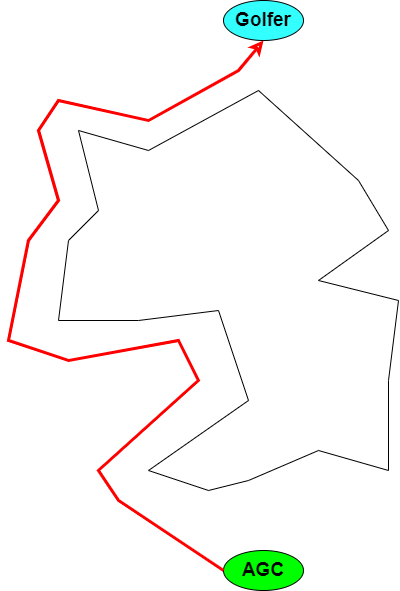
\includegraphics[width=0.65\textwidth]{padding.png}
        \end{center}
    \end{mdframed}
    \captionof{figure}{Path derived by ``padding'' polygon}
    \label{fig:padding}
\end{Figure}

A custom pathfinding algorithm was designed and implemented. The path it finds
is not the optimal solution, but it computes quickly and the path derived is
more efficient than using the ``padding'' method. Fig.
(\ref{fig:pathfinding_flow}) shows the main steps performed by the algorithm to
determine where the AGC should go.

\begin{figure}[H]
    \begin{mdframed}
        \begin{center}
            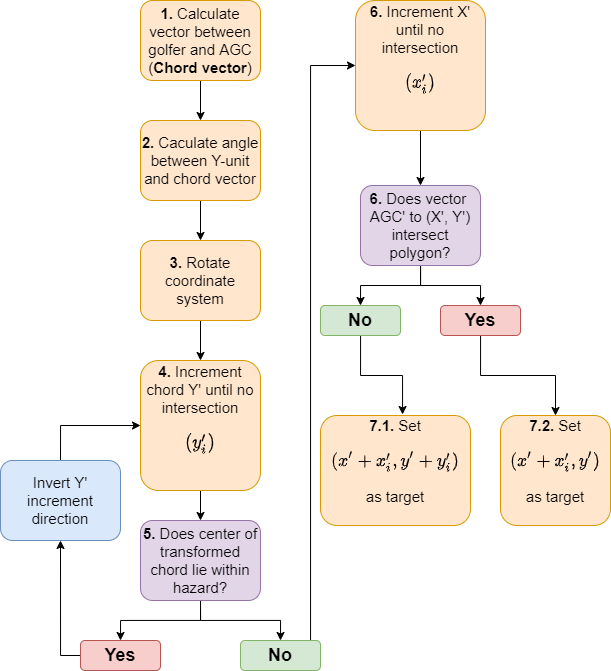
\includegraphics[width=0.95\textwidth]{pathfinding_flow.png}
        \end{center}
    \end{mdframed}
    \captionof{figure}{Pathfinding algorithm main steps}
    \label{fig:pathfinding_flow}
\end{figure}

First the chord vector, $\overrightarrow{\mathbf{C}}$, is calculated with Eq.
(\ref{eq:chord}) where $\overrightarrow{\mathbf{G}}$ is the golfer position and
$\overrightarrow{\mathbf{AGC}}$ is the AGC position. Also the angle, $\theta$,
between $\overrightarrow{\mathbf{C}}$ and the Y-unit vector, $\hat{\mathbf{y}}$,
is calculated using Eq. (\ref{eq:theta}).  The relevant polygon, golfer
position, and AGC position are rotated about the z-axis with the center of
rotation as the origin by $\theta$ using Eq. (\ref{eq:rotation_mat}) where
$\overrightarrow{p}$ is a three dimensional point and
$\overrightarrow{p^\prime}$ is the rotated point. The polygon is rotated by
applying Eq. (\ref{eq:rotation_mat}) to each vertex. The purpose of the rotation
was to aid the design process of the algorithm and make the code more readable,
removing the necesscity for vector manipulations throuhout the algorithm instead
using only simple arithmetic operations. This results in
$\overrightarrow{\mathbf{C}^\prime}$ having constant $y$. The value of
$y^\prime$ is incremented in one meter steps until no intersection between the
translated chord vector, $\overrightarrow{\mathbf{C}^\prime_t}$, and the rotated
polygon, $\mathbf{P}^\prime$. If any point of
$\overrightarrow{\mathbf{C}^\prime_t}$ lies within the polygon the increment
direction is reversed and incremented until there is no intersection and no
points of $\overrightarrow{\mathbf{C}^\prime_t}$ lie within the polygon. This
increment process is repeated in the $x^\prime$ direction for the vector joining
the rotated AGC position, $\left(x^\prime_{AGC}, y^\prime_{AGC}\right)$, to
$\left(x^\prime_{AGC}, y^\prime_{AGC} + y^\prime_i\right)$. Once the
incrementation process is finished such that no intersections are found, the
vector joining $\left(x^\prime_{AGC}, y^\prime_{AGC}\right)$ to
$\left(x^\prime_{AGC}+x^\prime_i, y^\prime_{AGC} + y^\prime_i\right)$ is checked
for intersections. If none are found then $\left(x^\prime_{AGC}+x^\prime_i,
y^\prime_{AGC} + y^\prime_i\right)$ is rotated back to the original coordinate
system and set as the position target for the AGC. If an intersection is found
then $\left(x^\prime_{AGC}+x^\prime_i, y^\prime_{AGC}\right)$ is rotated back to
the original coordinate system and set as the AGC position target. This process
repeats until the golfer is reached. Incrementing in the $y^\prime$ direction is
equivelant to incrementing perpendicular to $\overrightarrow{\mathbf{C}}$ in the
original coordinate system, and incrementing it by $x^\prime$ is equivelant to
incrementing in the direction of $\overrightarrow{\mathbf{C}}$.

\subsubsection{Target Reaching}
From our GPS module updated GPS can be acquired approximately once per
second. Between GPS readings, the enocders embedded in the EMG49 motors are used
to calculate the position of the AGC extrapolating from the total rotation of
the motors and the orientation of the AGC when the maneuver began. As soon as
new GPS data is available, the pathfinding algorithm will be run again, even if
the initial target location set by the algorithm has not yet been reached.
Running the algorithm more frequently results in a smoother path which sticks
closer to the perimeter of the polygon.

\begin{equation}
        \overrightarrow{\mathbf{C}} = \overrightarrow{\mathbf{G}} - \overrightarrow{\mathbf{AGC}}
    \label{eq:chord}
\end{equation}
\hspace{0.5cm}
\begin{equation}
        \theta=\operatorname{acos}\left(\frac{\overrightarrow{\mathbf{C}} \cdot \hat{\mathbf{y}}}{|\overrightarrow{\mathbf{C}}| |\hat{\mathbf{y}}|}\right)
    \label{eq:theta}
\end{equation}
\hspace{1cm}
\begin{equation}
    \overrightarrow{p^\prime} = \left(\begin{matrix}
        \operatorname{cos}\theta & -\operatorname{sin}\theta & 0 \\
        \operatorname{sin}\theta & \operatorname{cos}\theta & 0 \\
        0 & 0& 1\\
    \end{matrix}\right) \overrightarrow{p}
    \label{eq:rotation_mat}
\end{equation}
\hspace{0.5cm}
\begin{equation*}
    \overrightarrow{\mathbf{AGC}} = (x_{AGC}, y_{AGC})
\end{equation*}

\subsubsection{Pathfinding Diagram}
Fig. (\ref{fig:pathfinding_visual}) shows a visual of how the pathfinding
algorithm will determine intermediary positions for the AGC to move it towards
the golfer. For the generation of this figure the pathfinding algorithm was only
called again after the target position is reached, resulting in the very wide
path that can be seen in the final path diagram. On the AGC the pathfinding
algorithm is called every time new GPS data is available, approximately every
second, resulting in a smoother and closer path being found.
\end{multicols}
\newpage
\begin{figure}[H]
    \begin{mdframed}
        \begin{center}
            \begin{minipage}{0.3\textwidth}
                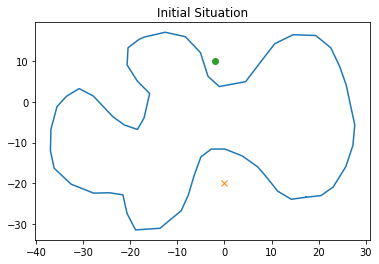
\includegraphics[width=0.95\textwidth]{initial.png}
            \end{minipage}
            \begin{minipage}{0.3\textwidth}
                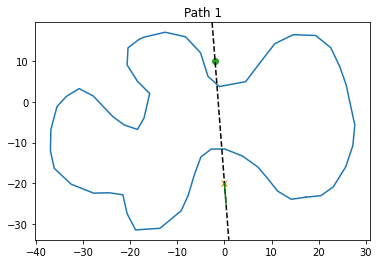
\includegraphics[width=0.95\textwidth]{p1.png}
            \end{minipage}
            \begin{minipage}{0.3\textwidth}
                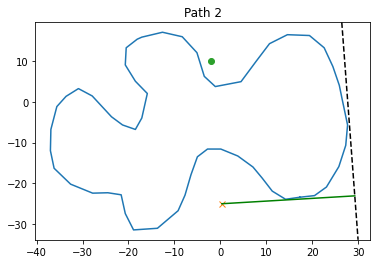
\includegraphics[width=0.95\textwidth]{p2.png}
            \end{minipage}
        \end{center}
        \begin{center}
            \begin{minipage}{0.3\textwidth}
                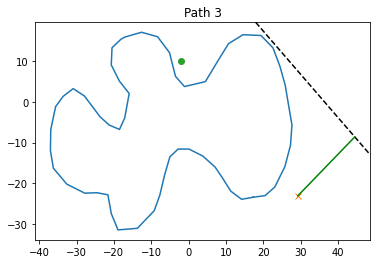
\includegraphics[width=0.95\textwidth]{p3.png}
            \end{minipage}
            \begin{minipage}{0.3\textwidth}
                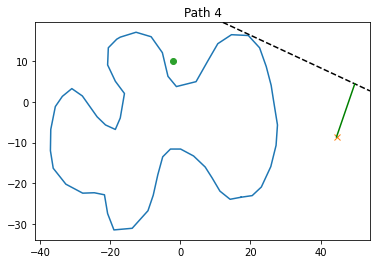
\includegraphics[width=0.95\textwidth]{p4.png}
            \end{minipage}
            \begin{minipage}{0.3\textwidth}
                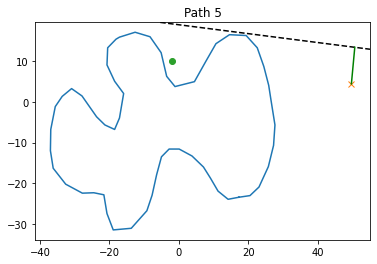
\includegraphics[width=0.95\textwidth]{p5.png}
            \end{minipage}
        \end{center}
        \begin{center}
            \begin{minipage}{0.3\textwidth}
                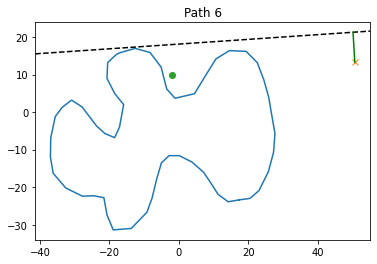
\includegraphics[width=0.95\textwidth]{p6.png}
            \end{minipage}
            \begin{minipage}{0.3\textwidth}
                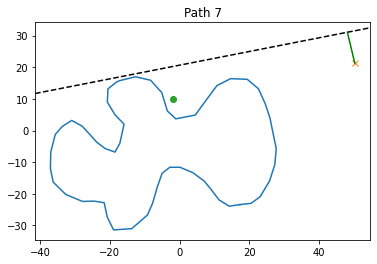
\includegraphics[width=0.95\textwidth]{p7.png}
            \end{minipage}
            \begin{minipage}{0.3\textwidth}
                \includegraphics[width=0.95\textwidth]{final.png}
            \end{minipage}
        \end{center}
    \end{mdframed}
    \captionof{figure}{Visualisation of path determined by pathfinding algorithm}
    \label{fig:pathfinding_visual}
\end{figure}
\newpage

\begin{multicols}{3}

\subsection{Communications}
The EMG49 motors used are controlled by the MD25 motor controller board
via serial communication. The communication interface for this was written
in C and is capable of handling multiple serial devices; if more than one device
is present the serial port can be closed and reopened rapidly. Currently the
only device on the communications network is the MD49. The GPS in the
golfer's pod communicates to the main Raspberry Pi via Bluetooth, which is
written in Python using the PyBluez library. The GPSs communicate with the
Raspberry Pis via serial commuication implemented using the Pyserial library,
using it's own designated serial port.


\subsection{GUI}

A graphic user interface (GUI) is a graphics-based operating system interface
that uses icons, menus and a mouse to manage interaction with the system. In
this project, a GUI was developed to enable interactions between the golfer and
the AGC, mainly for the golf suggestion system. The GUI would also act as an
information center to display all information relevant to the golfer’s
game which could include weather forecasts, GPS location and performance
analysis. However, the GUI in this project focused on making the system
interactive to enable the golfer to communicate with the AGC on the preferred
golf club in a round of golf. Based on the machine learning algorithm for the
golf suggestion system, the golfer would have the option to accept or reject the
suggested golf by interacting with the GUI, as shown in Fig. (\ref{fig:gui}),
and the result of the decision would be received by the golf suggesting
algorithm to improve its data and accuracy. 

\begin{figure}[H]
    \begin{center}
        \includegraphics[width=0.3\textwidth]{GUI.png}
    \end{center}
    \captionof{figure}{Flow chart of the golfer interacting with the AGC on a club suggestion through the caddy}
    \label{fig:gui}
\end{figure}

Initially the type of data representation that had to be displayed is peculiar
and there was no readily available software that could be used to implement
them. Therefore, a GUI had to be made from scratch in order to satisfy our aims
and objectives on the type of data representation. To display the GUI, options
such as LCD screen or even a phone app were considered. Frameworks that were
considered in order to make the GUI that could be represented on the options
above were Qt, Blynk IoT and React Native which is a library in JavaScript. Qt
was chosen due to its library in python called PyQt which would be easier to use
and considering that only a LCD touchscreen would be used, the user’s phone will
not have to be unusable whilst the GUI is on. 

\subsubsection{PyQt}
PyQt is mainly used for creating GUI, developing desktop applications with
Python. As an initial design implementation, the team decided to use PyQt as the
GUI because screen is able to showcase the GUI as an application through the
Raspberry Pi as its processor. The main reason PyQt is used for this project is
due to it being open source and provides many classes, methods and widgets. This
allows a rich app at not cost to be developed.  

There are two methods known to create a GUI through PyQt: a: through hard coding
i.e., manually coding the elements contained in the GUI and b: through a tool in
PyQt called QtDesigner which allows the user to pick and choose the elements
contained in the GUI. The second method is found to be easier as it allows the
user direct preview of how the GUI would look like. However, the drawback of
this method is that the user has less control of the GUI’s boundaries,
and an extra step is needed to convert the GUI from a user interface file (.ui)
to a python file to be used on python for the code (.py). The second method is
used with a combination of the first method for control of the boundaries. There
are a few GUIs created for the caddy with its use listed below in Table
(\ref{tab:gui_descs}) with its description.

\begin{table}[H]
    \begin{center}
        \resizebox{\columnwidth}{!}{%
        \begin{tabular}{|l|l|}
            \hline
            \textbf{GUI Name} & \textbf{Description} \\ \hline
            MyMap & \makecell{To showcase a virtual map of the golf course to indicate the\\
            live location of the AGC} \\ \hline
            MyGolf & \makecell{To allow the golfer to key in their information which \\
            includes age and skill level for the machine learning algorithm} \\ \hline
            MyClubs & \makecell{To allow the golfer to key in the information of the \\
            location of each club in each slots in the golf bag. This GUI also \\
            allows the golfer to interact with the caddy on whether they \\
            to use the recommended golf club or their own preference} \\ \hline
        \end{tabular}
        }
    \end{center}
    \captionof{table}{GUI names and descriptons}
    \label{tab:gui_descs}
\end{table}

After developing these GUIs, they were tested on the Raspberry Pi to see its
compatibility and functionality. All GUIs were working well and found compatible
with the Raspberry Pi. However, there were drawbacks on some of the
functionality of the GUI. First, MyMap was unable to generate a responsive map
that could allow the autonomous following algorithm to give and receive inputs
with the map. This is because PyQt and Python could not incorporate Google Maps
due to licensing and the alternative was a library from Python that could
generate a map which was Folium. Folium is a tool to visualise data that has
been manipulated through Python on an interactive leaflet. However, data from
the map could not be extracted to enable the autonomous following algorithm to
update the coordinates of the golfer and the AGC on the GUI. This results to a
static map that could only be updated when the coordinates are updated manually
in the algorithm. An alternative is to obtain the application programming
interface (API) and licensing from Google Maps and incorporate it into the GUI.
However, obtaining the API and licensing requires the team to purchase them at
a very high cost significantly beyond the budget allocated. Third and lastly,
MyGolf acts as key information for the golf suggesting algorithm because
information on the golfer’s age, gender and skill level are relevant for the
AGC to suggest a suitable golf club. 

Fig. (\ref{fig:MyMap}) shows the MyMap GUI containing a white space for where the map would be and information of the current hole with the distance between the golfer and the hole.

\begin{figure}[H]
    \begin{center}
        \includegraphics[width=0.2\textwidth]{MyMap.png}
    \end{center}
    \captionof{figure}{MyMap containing a white space for where the map would be and information of the current hole with the distance between the golfer and the hole}
    \label{fig:MyMap}
\end{figure}

Fig. (\ref{fig:MyGolf}) shows the MyGolf GUI displaying the current hole and the distance to the hole. This GUI would also be where the golfer would accept or reject the golf club suggested by the GUI.

\begin{figure}[H]
    \begin{center}
        \includegraphics[width=0.2\textwidth]{MyGolf.png}
    \end{center}
    \captionof{figure}{MyGolf shows the current hole and the distance to the hole. This GUI would also be where the golfer would accept or reject the golf club suggested by the GUI}
    \label{fig:MyGolf}
\end{figure}

Fig. (\ref{fig:MyClubs}) shows the MyClubs GUI that allows the golfer to input the golf club to the intended positions in the golf bag for the release mechanism.

\begin{figure}[H]
    \begin{center}
        \includegraphics[width=0.2\textwidth]{MyClubs.png}
    \end{center}
    \captionof{figure}{MyClubs allows the golfer to input the golf club to the intended positions in the golf bag for the release mechanism}
    \label{fig:MyClubs}
\end{figure}

\subsubsection{Course Map}
The course map was implemented on the GUI using the map system that was used on
the simulator. An attempt was made to embed a map in a web app called folium which looks
better than the map developed for the simulator, however, it did not allow
extraction of coordinates for a point clicked on the map in real latitude / longitude
coordinates or in screen coordinates. This shortfall makes it impossible to give
the golfer the ability to click a point on the map and see how far away it is
from the AGC, whereas using the simulator app, it was possible to add that feature.

\section{Course Geo-mapping}
The core of the autonomous following for the golf caddy as it is dependent on the
golf course data to know where the unallowed and hazardous areas are with high
accuracy. This is best done by using the GPS coordinates of the locations as it
pinpoints exactly where these locations are and enables the AGC to know where
the points are given that the coordinates are programmed into the autonomous
following algorithm.

The Southampton Municipal Golf Course was chosen as the project’s test site on
the grounds that it has a fair number of bunkers, greens and water which provide
good amount of data without being too overwhelming. It is also logistically
practical for testing as it accessible at a low cost. To ensure that the data
obtain was accurate, the data obtained is compared with Google Maps and a golf
app, VPAR which contains the number of greens according to its respective holes
and the relative coordinates of all locations. The comparison was found to be
accurate and helps strengthens the case of choosing the GPS coordinates of the
unallowed and hazardous locations as the data source for the autonomous
following system. 

The best way to extract the coordinates that allow the AGC to understand which
area it should avoid is by drawing out polygon maps through the perimeters of
the unallowed and hazardous locations. By doing this, it saves time and reduces
computational speed as it does not require to extract every single point within
the area (for accuracy) and the algorithm for the autonomous following would not
have to go through so many data that would be costly in computational speed. For
accuracy, the polygons drawn as the perimeter would need to be as close as possible
to increase the points within the perimeter of the area that the AGC should avoid.

The coordinate is then extracted from a feature of this software which allows it
to be formatted as a text file. As mentioned, the waypoints were drawn as
closely to each other as possible. Fig. (\ref{fig:mission_planner}) illustrates
the Southampton Municipal Golf Course on Mission Planner. The Mission Planner
and Google Maps were found to be both identical and all coordinates match with
each other on the maps. Prohibited zones are then created by drawing constructing
a polygon formed by clicking points of the perimeter of a zone that the AGC should
not trespass onto; the concept is demonstrated in Fig. (\ref{fig:polygon1}).

\begin{figure}[H]
    \begin{center}
        \includegraphics[width=0.3\textwidth]{Municipal.png}
    \end{center}
    \captionof{figure}{Mission Planner view of Southampton Municipal Golf Course}
    \label{fig:mission_planner}
\end{figure}

\begin{figure}[H]
    \begin{center}
        \includegraphics[width=0.3\textwidth]{polygon 1.png}
    \end{center}
    \captionof{figure}{Mission Planner view of Southampton Municipal Golf Course}
    \label{fig:polygon1}
\end{figure}

Ultimately, the goal of course geo-mapping is to obtain all the coordinates of the
perimeter of all unallowed and hazardous areas on the golf course. Subsequently, the
coordinates would be extracted and used for the autonomous following system.

\section{Electronics}
\label{electronics}
\subsection{AGC On Board Electronics}
The trolley will be having a raspberry pi as a microcontroller, two EMG49
motors, an MD49 motor driver, three stepper motors with three A4988 stepper
drivers, a GPS module, a 24v battery and a touchscreen display.

\subsubsection{Processing Unit}
For the trolley microcontroller, the Raspberry Pi 4B with 4 GB of RAM will be
used. Other affordable alternatives of microcontrollers are Arduino boards.
However, the Raspberry Pi is chosen because of its superiority in processing
power, its easy compatibility with touchscreen displays and in-built Wi-Fi
module allowing the possibility to work with APIs and remotely access the system
through SSH. The microcontroller will also have a set of heat sinks plus a fan
that will avoid any overheating problems.


\subsubsection{Motors}
The EMG49 motors were chosen for the prototype. These motors were selected by
considering the desired top speed of the AGC, and the desired time for it
to accelerate to that speed on a $10^\circ$ incline. The calculations shown
below in Fig. (\ref{fig:motor_calcs}) show how calculations of the necessary
torque and rpm required from the motors.

\begin{figure}[H]
    \begin{mdframed}
        The desired top speed for the AGC was 5.0 kilometers per hour,
        equivalent to average walking speed. The wheel radius, $W_r$ of the AGC
        wheels is 0.115 meters. Required RPM is calculated with Eq. (\ref{eq:rpm}):
        \begin{center}
            \begin{equation}
                rpm = \frac{7.5 * \frac{1000}{3600}}{2\pi W_r} \cdot 60 \approx 115rpm
                \label{eq:rpm}
            \end{equation}
        \end{center}
        The AGC should be able to accelerate to this speed, $V$, within $t=5$
        seconds on a $10^\circ$ incline. For predicted final mass, $M = 15kg$,
        the accelerating force, $F$, required can be calculated with Eq.
        (\ref{eq:accel}):
        \begin{center}
            \begin{equation}
                F = M\frac{V}{t} + M g_0 \sin(10^\circ)\approx 29 N
                \label{eq:accel}
            \end{equation}
        \end{center}
        Finally the torque required from each motor can bel calulated using Eq.
        (\ref{eq:torque}):
        \begin{center}
            \begin{equation}
                T = W_r * \frac{F}{2} \approx 1.7 Nm
                \label{eq:torque} 
            \end{equation}
        \end{center}
    \end{mdframed}
    \captionof{figure}{Motor requirement calculations}
    \label{fig:motor_calcs}
\end{figure}

According to their datasheet the EMG49 motors can provide a loaded rpm of 122
and a torque of 1.56, close to our requirements set out above. As the torque is
slightly lower than calulated, the AGC will accelerate slightly to top speed on
a $10^\circ$ incline in slightly over five seconds.

Shown in Fig. (\ref{fig:emg49}), is a 24v motor fully equipped with
encoders and a 49:1 reduction gearbox. It is ideal for medium to large robotic
applications, providing cost effective drive and feedback for the user. It also
includes a standard noise suppression capacitor across the motor windings
\cite{emg49data}.
\begin{figure}[H]
    \begin{center}
    \includegraphics[]{emg49.png}
\end{center}
\captionof{figure}{EMG49 Motor}
\label{fig:emg49}
\end{figure}

\subsubsection{MD49 Motor Controller}
The MD49 motor driver, as shown in Fig. (\ref{fig:electrical_schematic}), is a
robust serial dual motor driver, designed for use with the EMG49 motors. Its
main features are \cite{md49data}:

\begin{itemize}
    \item Reads motors encoders and provides counts for determining distance traveled and direction of rotation.
    \item Drives two motors with independent or combined control. 
    \item Motor current is readable.
    \item Only 24v is required to power the module.
    \item Variable acceleration and power regulation also included
    \item Protection against short circuit and incorrect voltage. 
    \item An error byte can be read to aid troubleshooting.
\end{itemize}

\subsubsection{Stepper Motors}
The release mechanism requires a low RPM and high torque (minimum of 0.13 Nm)
motor to push harder from rest. The ones used and shown in Fig.
(\ref{fig:electrical_schematic}) are the NEMA 17 stepper motors. They have a
maximum holding torque of 0.53 Nm, a rated voltage of 12-24V and require 1.5A
per phase so 3A per motor. 

\subsubsection{A4988 Stepper Motor Driver}
The A4988, shown in Fig. (\ref{fig:stepper_driver}), is a high-performance
stepper motor driver that allows an easy control of one bipolar stepper motor up
to 2A output current per coil. It comes with a heatsink as it can potentially
reach 150$^{\circ}$ \cite{stepper_driver}.
Its operating voltage lies in the range of 8 to 35 V. According to the driver
specification, the stepper motor supply requires a 100µF decoupling capacitor
close to the driver to sustain 4A. This capacitor is shown in Fig.
(\ref{fig:electrical_schematic}).

\begin{figure}[H]
    \begin{center}
    \includegraphics[]{stepper_driver.jpg}
    \captionof{figure}{A4988 Stepper Motor Driver}
    \label{fig:stepper_driver}
    \end{center}
\end{figure}

\subsubsection{GPS Module}
The GPS module called NEO-6M shown in Fig. (\ref{fig:gps_module}) can sense
locations through the whole world by tracking 22 satellites. It takes 27 seconds
to start accurately, provides GPS data in the form of NMEA sentences, and
requires very little power with only 3.3V at 45mA necessary \cite{neo_gps}.

\begin{figure}[H]
    \begin{center}
        \includegraphics[]{gps_module.png}
        \captionof{figure}{GPS Module}
        \label{fig:gps_module}
    \end{center}
\end{figure}


\subsubsection{Power Supply}
The power for the trolley will be supplied by four packs filled with eight AA
1.5V 3Ah batteries. The configuration consists in two pairs of packs in
parallel, resulting in a final configuration of 16s2p of AA cells. This is shown
is Fig. (\ref{fig:electrical_schematic}). As a result, the total supply of
voltage is of 24V with a capacity of 6Ah. Initially, the trolley had EMG30
motors rated at 12V and powered by a 12V 16Ah lithium battery inherited from the
supplied trolley. However, the late upgrade in DC motors forced the group to
change the battery to meet the required 24V the new motors needed. Lacking in
budget, the only alternative was to use 32 AA batteries. During testing it was found
that this configuratin was unable to supply enough current to the motors,
resulting in the motors unable to run at maximum speed. As out goal was simply
to demonstrate the AGC abilities, it was not necessary for the AGC to operate at
maximum speed. Were a final product to be manufactured then a more
appropriate solution to power the system would be required.

As shown in Fig. (\ref{fig:electrical_schematic}), the first components after
the battery are a 5A fuse and a switch to turn on/off the whole trolley. These
are wires were soldered directly without a base, so an insulated rubber has been
heat-shrinked to avoid short circuits. After this, a stripboard with a 5V and 5A
voltage regulator, shown in Fig. (\ref{fig:voltage_regulator}),
reduces the voltage to 5V. These 5V power the raspberry pi, the GPS module, the
3 A4988 Vcc logic input and the touchscreen. The stepper and DC motors are
powered with 24V so do not need a regulated voltage. 

\begin{figure}[H]
    \begin{center}
        \includegraphics[]{voltage_regulator}
        \captionof{figure}{Voltage Regulator}
        \label{fig:voltage_regulator}
        \end{center}
\end{figure}

\subsubsection{Touchscreen Display}
The touchscreen used is a 5-inch DSI capacitive touch display. It was chosen
because of its convenient connection to the raspberry pi, which only consist of
a ribbon, and its affordable price. It also brings mounting holes and screws to
fit it in a case as was done on the AGC shown Fig. (\ref{fig:holder}). 

\subsection{Pod Electronics}
The pod, which is used to make the trolley follow the user via GPS, contains
another Raspberry Pi and a GPS module with a 9V battery.
\subsubsection{Microcontroller}
Again, a Raspberry Pi 4B (RP4B) will be used as a microcontroller thanks to its
in-built Bluetooth module which easily allows a connection between two raspberry
pi’s within a range of 240m, allowing the user to separate from the caddie no
more than this distance \cite{raspi}.
The size of the pod can be decreased by using a Raspberry Pi Zero as a
microcontroller instead of the RP4B. This is because the Zero version is much
smaller, has the same built-in Bluetooth and Wi-fi range connection and consumes
only 120mA on idle compared to a higher 540mA for the RP4B. As a result, a
smaller battery would be required, decreasing the overall size, and improving
the customer experience since the smaller and more versatile the pod is, the
more comfortable it will be to keep it in the pocket or other place. However,
due to the worldwide microprocessor manufacturing shortage, there has not been
any available stock for a long time, hence, the use of the groups owns Raspberry
Pis. 

\subsubsection{Power Supply}
The power of the pod is supplied by a 9V 0.4Ah battery. It also contains a
switch to turn on/off the whole pod.

\end{multicols}

\begin{figure}[H]
    \begin{center}
    \includegraphics[width=0.8\textwidth]{electrical_schematic.png}
    \captionof{figure}{Electrical Schematic}
    \label{fig:electrical_schematic}
    \end{center}
\end{figure}

\begin{multicols}{3}

\newpage
\section{Optimal Club Prediction}
One of the main aspects of the project that involved innovation consisted in
building a release mechanism that could offer a single golf club to the player
that would stand out from the rest due to its height difference in the golf bag.
Hence, an algorithm that would suggest for every shot the best club had to be
created. A golf game only allows fourteen golf clubs to be used and a single
club per shot. The selection of the golf club depends on the specific
circumstances to each shot.

The AGC will have the option to enable the optimal club choice predictions if
the user desires it. This option is placed on the AGC because current golf
regulations outside the United States do not permit the use of software to help
the golfer.

\subsection{Big Data against simulation and empirical data}
At the first project stages, it was assumed the data to train the algorithm
could exist online for free. However, only paid database that contained the name
and location of all golf courses throughout the world exists. As much as this
database would still help to gather data for other aspects of the project, it
was not worth buying it due to the high price and irrelevancy to improve a
golf club recommendation algorithm.

Hence, the group was left with 3 remaining options. The first option consists in
creating a very realistic simulation that emulates a golf shot while considering
as many variables as possible. The second option consists in having all the team
members to meet in a golf course and simply play the sport while gathering as
much data as possible. Lastly, the third option consist in creating a synthetic
database. Synthetic data is annotated information that computer simulations or
algorithms generate as an alternative to real-world data. The group would create
the data by researching and doing educated guesses to create relationships
between variables that approximate to the ones in real life as much as possible.

To create a real-life simulation, the physical interactions between all possible
variables, most importantly, the material interaction between the club and the
ball, would have to be considered. Other interactions to simulate would be how
wind direction; wind speed and air temperature change the golfs ball trajectory
by acting on its drag. Furthermore, the force magnitude used to hit the golf
ball by a person based on their age and gender would also have to be known,
hence complicating the task even more. This simulation could be done by using
mathematical equations and performing numerical methods to solve each equation.
However, the result of this idea would lead to an everlasting program that could
never be perfect due to the mathematical models always being approximations to
the real world. More importantly, the computational power and knowledge required
to build such simulation is far out of the scope of this project. 

On the other hand, using empirical data collected by playing actual golf in a
course would make the data as realistic as it can get. However, two main
inconveniences prevented this this option. First, all the team members from
this GDP fit into the same demographic in terms of gender, age, and experience
with golf. Hence, the collected data would have been too skewed against our
averages making the extrapolation inaccurate. Secondly, even if the groups
gender, age, and golf experience was more distributed, each member would have to
pay to play in the golf course, increasing the budget of the project.

As result of both options not being viable for this project, the group went on
to build a synthetic database since it is the most practical option considering
the resources available.

\subsection{Dataset generation}
A synthetic database was created with Python since it has very easy modules to
handle data. The resulting database consist of thirty-three thousand rows and
eighteen columns. Table (\ref{tab:guillermo_t3}) shows six randomly selected rows from the entire
database with their respective values and columns.

\subsection{Input Data}
The input data will be the data used to train the model. Machine learning models
are only as good as the data you use to train the model, hence the more data and
the more accurate the better for the model. This is the reason the synthetic
database must be carefully created, so that the AGC suggests for each shot the
correct golf club eventually satisfying the customer and being able to replace a
caddie.

A list taken from the most frequent male and female English names in the UK was
taken to create over more than 200 fake identities with their respective gender;
random age within a sensible range of 10 to 75 years old; a random skill level,
where the options can be beginner, average, good and excellent. As much as the
model would improve by asking even more personal information such as the diet
the user has, number of sleeping hours, heart rate and years of golf training, a
point will be reach were the user becomes dissatisfies by the amount data they have
to manually fill into the GUI or reject to fill the information as it is
personal and private. Therefore, the gathering of personal data has been limited
to only the basics.

After the 200 identities were created, a double for loop is used to iterate
through all the possible golf club types and choose the number of times a person
shot a ball with each different club. Assuming ten shots per type of club, it
leads to a total of approximately thirty thousand different shots with each one
being very likely to be unique. 

Column number five specifies the handicap of each identity. This has been
calculated by considering the gender, whether the user is over 19 years old and
its skill level. Each possible combination of these three parameters will have a
random number extracted from different normal distributions where each
distribution has an average taken from external sources and an educated guessed
standard deviation. From Lawrence \cite{golf_charts} two tables were imported to
help the database approximate to reality even more. The two tables, one for male
and another for female, consisted in the average distance a golfer hits a golf
ball depending on a variety of sixteen clubs with different loft angles and four
levels of skill. This can be shown in Table (\ref{tab:guillermo_t1}). By
allocating each identity to its respective cell in Table
(\ref{tab:guillermo_t1}), where gender and type of club chosen should match,
a random number from a normal distribution can be chosen. The normal
distributions mean is the average distance each identity fits according to their
gender and club, and the standard deviation is the average between the upper and
lower cell difference to the centre cell. 

In addition to the linear distance, an actual distance was also incorporated
into the database shown by column seven in Table (\ref{tab:guillermo_t3}). In
golf, although a player may know the exact distance, he wants to hit the ball,
the actual distance ends up being different depending on many parameters. To
artificially simulate how these parameters affect the ball trajectory, a
function was developed which considers the linear distance, the mean and
standard deviation of each identity and club, the wind speed, the temperature,
the elevation above sea level of the golf course and the height difference
between the player and its aimed location to hit the ball. Firstly, the better
the skill level of the identity, the lower the coefficient that multiplies the
standard deviation meaning that better players will show a lower range of values
than the others. This is shown in Fig. (\ref{fig:distribution}), where the
standard deviation of each normal distribution is seen to decrease as the player
has higher skill level. The wind speed is also multiplied to the standard
deviation, so that the higher the wind speed, the higher the possibility of the
balls trajectory ending up further than expected. Moreover, according to a study
by Trackman, a company specialising in golf simulation, atmospheric conditions
affect the actual distance in the following ways; for every ten degree decrease
in temperature, the ball will be carried 2.5 yards shorter and for every 1000
feet increase above sea level, the ball will be carried an extra 4.5 yards.
Furthermore, the elevation difference between the player position to the aimed
location is also considered for the actual distance. This time, the elevation is
added to the actual distance, so if the desired location is 4 meters
above the players location, the actual distance will be 4 meters shorter. All of
these relationships have been used to simulate the actual distance each identity
would hit. Fig. (\ref{fig:distribution}) shows the actual distance and compares
it to the linear distance. 

\begin{Figure}
    \begin{center}
        \includegraphics[width=0.8\textwidth]{distribution.png}
        \captionof{figure}{Frequency of shot distance with driver for adult males at different levels}
        \label{fig:distribution}
    \end{center}
\end{Figure}

As a result of the actual distance being approximating more to real life
conditions, another column was created in the database which corrects the club
that the user should have taken had he not considered only the distance.
Moreover, the variables wind speed and golf course elevation are random numbers
extracted from a gamma distribution with sensible means and standard deviation
to increase the realism in the synthetic database, since both continuous
variables follow this distribution in the real world \cite{wind_dist}. 



\subsection{Output Metrics}
The main aim of the AGC is to essentially behave as close as possible to a
real-life caddie. This means helping the user improve its game while also
carrying its golf bag and extra equipment. As a result, the AGC should be able
to offer data analytics for each user. These analytics should provide useful
insights that allows the player to leverage them and improve its golf
statistics. Furthermore, with the ever-increasing sport analytics market,
projected to be valued at USD 5.11 billion by 2026,
more and more users will be demanding this characteristic in the AGC \cite{analytics}. 

In Table (\ref{tab:guillermo_t3}), it can be seen two variables in the unit degrees called aimed
direction and wind direction. Since both are bearings, the nearest angle between
both has been calculated and created a third and fourth variable called angle of
deviation and tendency. Angle of deviation describes the difference in angle to
which the balls trajectory differs from the required path and tendency shows in
words where the ball landed relative to the aimed direction. From this data, the
performance of a player to deliver the ball where he aims can be assessed by
creating a scatter plot with polar coordinates where $\theta$ is the angle of
deviation and radius, $r$, is the missed distance. Together, the AGC can make the
user visualize via the screen this plot and find hidden patterns. For example, a
player may have tendency to hit the ball to the left side in certain holes of
the golf course, as shown in Fig. (\ref{fig:compass}) below. 

\begin{figure}[H]
    \begin{center}
        \includegraphics[]{compass.png}
    \end{center}
    \captionof{figure}{Golfer shot pattern graphic}
    \label{fig:compass}
\end{figure}

\subsection{Prediction Algorithm}
\subsubsection{Introduction}
Predictive modelling can be described as the mathematical problem of
approximating a mapping function, $f(x)$ from input variables $x$ to output
variables, $y$, to find the function approximation given the time and resources
available. For the AGC model, the input variables are all of the columns from
Table (\ref{tab:guillermo_t3}) except `actual club' and y is the actual club
variable \cite{classvsreg}.

To select the optimal algorithm to predict the optimal club choice, a series of
characteristics from the synthetic data set must be considered. First, identify
whether the training dataset has labelled data. Labelled data is a designation
for pieces of data that have been tagged with one or more labels identifying
certain properties or characteristics \cite{labeled_data}. Machine learning
algorithms can be classified into supervised and unsupervised. If the data is
labelled, which is the case for the synthetic database, the selected algorithm
must be of the type supervised. The reason it is called supervised learning is
because at least part the approach requires human oversight. On the other hand,
unsupervised learning trains models with raw and unlabelled data to cluster and
analyse datasets. 

Supervised machine learning is used to classify unseen data into establish
categories and forecast trends and future change as a predictive model. It will
learn to recognise object and the features that classify them by learning
patterns between input and output data \cite{seldon}. The two
types of supervised models are classification and regression. 

\subsubsection{Classification or Regression}
Regression models require the prediction of a continuous quantity while
classification require the prediction of discrete variables. Classification
models can be divided into binary or multiclass problems, where binary predict
only a category out of two and multiclass predicts more than one category. The
AGC model intends to forecast the optimal type of golf club, i.e., sixteen
different categories, so only multiclass classification algorithms are
considered. 

However, in some cases, such as the AGC case, classification algorithms can be
converted to regression problems. As shown in Table (\ref{tab:guillermo_t3}), some data types are in
the form of words. The data used to train the model has to be numerical. Hence,
the data must be pre-processed before inputting it. This is done by encoding
each variable either ordinally, nominally or binary. Ordinal encoding involves
mapping each unique label to an integer value and will only work if there is a
known relationship between the categories. For the club choice and skill level
variables, an ordinal relationship exists because from the lob wedge to the
driver the average distance increases and from beginner to expert the experience
also increases. Other word variables such as tendency are nominally encoded
since no relationship exist between them. Once the categorical data is encoded
it can be converted to a continuous range. Binary encoding works with the
variable gender, where male is 1 and female is 0.

As a result, both types of supervised algorithms are tested to compare their
performance and choose the optimal.

\subsection{Performance Assessment}
Python programming with the imported module scikit-learn was used to write all
machine learning algorithms. The synthetic database must first be randomly
divided into training data and test data. The model will be trained with the
training data and validate its prediction with the test data. For all the
algorithms, 10\% is used to test and 90\% to train. After the database has split,
the model is trained, validated, and finally analysed for its performance.

The process to choose the optimal algorithm consist in testing the most popular
algorithms and evaluating their performance by comparing the results. Table (\ref{tab:guillermo_t2})
shows the performance of the tested algorithms. For classifiers, the performance
is measured by the accuracy score, which computes the ratio between true
positives and all other predictions. If ${\hat{y}}_i$ is the predicted value of
the $\mathcal{i}_{th}$ sample and $y_{\mathcal{i}}$ is the corresponding true value,
then the fraction of correct predictions over $n_{samples}$ is defined as shown
in Eq. (\ref{eq:classifier_accuracy}).

\begin{equation}
    \textrm{accuracy } (y, \hat{y})=\frac{1}{n_{samples}} \sum_{i=0}^{n_{samples} - 1} 1(\hat{y}_i=y)
    \label{eq:classifier_accuracy}
\end{equation}

Where 1(x) is the indicator function \cite{scikit}. For
regression, performance is measured by computing $R^2$ (coefficient of
determination), which assesses the ability of a model to predict or explain an
outcome in the linear regression setting. The best value is 1.0 and it can be
negative because the model can arbitrarily be worse. If ${\hat{y}}_i$ is the
predicted value of the $\mathcal{i}-th$ sample and $y_{\mathcal{i}}$ is the
corresponding true value for n samples, the estimated $R^2$ is defined as shown in
Eq. (\ref{eq:regression_accuracy}).
\begin{equation}
        R^2(y,\hat{y})=1 - \frac{\sum_{i=1}^{n}(y_i-\hat{y}_i)^2}{\sum_{i=1}^{n}(y_i-\overline{y}_i)^2}
    \label{eq:regression_accuracy}
\end{equation}

Where:
\begin{equation*}
        \overline{y} = \frac{1}{n}\sum_{i=1}^{n}y_i \textrm{ and } \sum_{i=1}^{n}{y_i - \hat{y}_i} = \sum_{i=1}^{n}\epsilon^2
\end{equation*}

Also, the MAPE (mean absolute percentage error) is measured for regression. This
metric computes the absolute error for every prediction and returns its mean. If
${\hat{y}}_i$ is the predicted value of the $\mathcal{i}_{th}$ sample and
$y_{\mathcal{i}}$ is the corresponding true value, then the mean absolute percentage
error estimated over $n_{samples}$ is defined shown in Eq. (\ref{eq:mape}).

\begin{equation}
        MAPE(y,\hat{y})=\frac{1}{n_{samples}}\sum_{i=0}^{n_{samples} - 1}\frac{\left|y_i - \hat{y}_i\right|}{\max(\epsilon,|y_i|)}
        \label{eq:mape}
\end{equation}

where $\epsilon$ is an arbitrary small yet strictly positive number to avoid
undefined results when y is zero
\cite{scikit}.

Table[2] also shows how much time the algorithm takes to execute. As a result of
taking all metrics into consideration, and prioritising the accuracy more than
the execution time, the chosen model is a random forest classifier. It has the
highest accuracy and although the execution time is of one minute, this does not
mean the user will have to wait one minute every time he wants to get a
suggested golf club. Hence, the AGC will recommend the optimal golf club 96\% of
the time as shown in Table (\ref{tab:guillermo_t2}).



\end{multicols}
\newpage
\begin{table}
    \centering
    %\resizebox{\columnwidth}{!}{%
    \begin{tabular}{|l|l|l|l|l|l|l|l|l|}
        \hline
                   & Male     &         &        &           & Female   &         &        &           \\ \hline
    Club           & Beginner & Average & Good   & Excellent & Beginner & Average & Good   & Excellent \\ \hline
    Driver         & 137.1   & 160.0     & 182.8 & 210.2    & 173.7   & 201.1  & 228.5 & 255.9    \\ \hline
    3 Wood         & 114.3   & 137.1  & 164.5 & 192.0       & 155.4   & 192.0     & 205.7 & 214.8    \\ \hline
    5 Wood         & 100.5   & 128.0     & 160.0    & 182.8    & 137.1   & 178.2  & 187.4 & 201.1    \\ \hline
    Hybrid         & 96.0       & 123.4  & 155.4 & 178.2    & 132.5   & 164.5  & 173.7 & 192.0       \\ \hline
    2 Iron         & 96.0       & 123.4  & 155.4 & 173.7    & 132.5   & 164.5  & 173.7 & 196.5    \\ \hline
    3 Iron         & 91.4    & 114.3  & 146.3 & 169.1    & 123.4   & 155.4  & 164.5 & 187.4    \\ \hline
    4 Iron         & 82.3    & 109.7  & 137.1 & 164.5    & 114.3   & 146.3  & 155.4 & 178.2    \\ \hline
    5 Iron         & 73.1    & 100.5  & 128.0    & 155.4    & 109.7   & 141.7  & 150.8 & 169.1    \\ \hline
    6 Iron         & 64.0       & 91.4   & 118.8 & 146.3    & 105.1   & 132.5  & 146.3 & 160.0       \\ \hline
    7 Iron         & 59.4    & 82.3   & 109.7 & 137.1    & 96.0       & 128.0     & 137.1 & 150.8    \\ \hline
    8 Iron         & 54.8    & 73.1   & 100.5 & 128.0       & 86.8    & 118.8  & 128.0    & 141.7    \\ \hline
    9 Iron         & 50.3    & 64.0      & 86.8  & 118.8    & 73.1    & 105.1  & 114.3 & 132.5    \\ \hline
    Pitching Wedge & 45.7    & 54.8   & 73.1  & 105.1    & 64.0       & 91.4   & 100.5 & 123.4    \\ \hline
    Gap Wedge      & 41.1    & 50.3   & 64.0     & 86.8     & 54.8    & 82.3   & 91.4  & 114.3    \\ \hline
    Sand Wedge     & 36.6    & 45.7   & 54.8  & 77.7     & 50.3    & 73.1   & 86.8  & 105.1    \\ \hline
    Lob Wedge      & 32.0       & 41.1   & 45.7  & 64.0        & 36.6    & 54.8   & 73.1  & 96.0        \\ \hline
    \end{tabular}%
    %}
    \captionof{table}{Average shot distance (in metres) with different clubs for men and women of different skill levels}
    \label{tab:guillermo_t1}
\end{table}
    
\begin{table}
    \centering
    \begin{tabular}{|l|l|l|l|}
        \hline
    Algorithm name &                &      &                     \\ \hline
    Classifiers    & Accuracy score (\%) &      & Execution Time (s)  \\ \hline
    KNN            & 0.21           &      & 1.80                 \\ \hline
    Decision Tree  & 0.22           &      & 0.04                \\ \hline
    Naives Bayes   & 0.23           &      & 0.02                \\ \hline
    Kernel SVM     & N/A            &      & Too long            \\ \hline
    Random forest  & 0.96           &      & 58.80                \\ \hline
                   &                &      &                     \\ \hline
    Regression     & R\^{}2         & MAPE &                     \\ \hline
    Linear         & -43            & 0.47 & 0.07                \\ \hline
    Decision Tree  & 0.86           & 0.09 & 0.23                \\ \hline
    Random forest  & 0.92           & 0.08 & 145.00                 \\ \hline
    Neural network & -3.00             & 0.42 & 3.62                \\  \hline
    \end{tabular}
    \captionof{table}{Performance metrics of various machine learning algorithms}
    \label{tab:guillermo_t2}
\end{table}
    
\begin{table}[H]
    \centering
    \begin{tabular}{|l|l|l|l|l|l|l|l|l|l|l|l|l|l|l|l|l|l|l|}
        \hline
           & username & age & gender & skill\_level & handicap & linear\_dist & actual\_dist & missed\_dist & club   & actual\_club & aimed\_dir & wind\_dir & ws   & angle\_dev & tendency  & temp  & height\_above\_sea\_level & elev\_diff  \\  \hline
    28,701 & Kathryn  & 19  & Female & Average      & 21       & 96.90        & 110.70       & 13.80        & 4 Iron & 6 Iron       & 51         & 191       & 9.40 & 94.10      & right     & 29.30 & 180.60                    & -10         \\ \hline
    25,065 & Heather  & 68  & Female & Excellent    & 2        & 133.60       & 128.30       & 5.30         & 8 Iron & 8 Iron       & 215        & 136       & 3    & 2.40       & top       & 5.60  & 356.40                    & -2          \\ \hline
    11,524 & Roger    & 51  & Male   & Average      & 24       & 203.50       & 231.40       & 27.90        & Driver & Driver       & 77         & 259       & 4.70 & 55.50      & top right & 29.70 & 473.10                    & -6          \\ \hline
    4,838  & Edward   & 68  & Male   & Good         & 12       & 191.10       & 181.70       & 9.40         & Hybrid & 5 Wood       & 171        & 206       & 3.10 & 14.90      & top right & 27.80 & 435.90                    & 8           \\ \hline
    18,352 & Sarah    & 44  & Female & Excellent    & 3        & 100.40       & 128.30       & 27.90        & 9 Iron & Gap Wedge    & 280        & 96        & 3.90 & 360.60     & top       & 17.50 & 700.70                    & 0           \\ \hline
    22,344 & Angela   & 40  & Female & Excellent    & 6        & 138.30       & 140.50       & 2.20         & 8 Iron & 7 Iron       & 38         & 79        & 3.20 & 305.70     & top left  & 21.90 & 779.80                    & 5           \\ \hline
    \end{tabular}
    \captionof{table}{Sample synthetic data}
    \label{tab:guillermo_t3}
\end{table} 


\newpage
\begin{multicols}{3}
\subsection{Future Work}
Despite the fact the model has great accuracy, in the end, the model will be as
good as its data. In the future, before commercialising the product, empirical
data from players with a range of abilities and identities should play with the
AGC to gather real data and verify the synthetic database precision.

\subsubsection{APIs}
When in commercialization or in testing stage, the weather and physical
conditions that exist in the synthetic database will be recorded thanks to two
APIs (application programming interfaces) that require a hotspot connection from
the users phone, which the Raspberry Pi can connect to.

\paragraph{GCP Elevation API} 
The elevation is needed because the height difference in golf shots is relevant
to decide the optimal club choice. Hence, the first idea was to use a Google
Cloud Platform (GCP) elevation application programming interface (API). The
platform allows a free trial period and after this the price per 1000 request is
of 4-5 US dollars \cite{google_docs}. 

Having the location of the pod, which will be carried by the user, and the
location of the hole in the golf course, the height difference can be known by
transforming the location into latitude and longitude coordinates and requesting
the call from the API

\paragraph{Openweather API}
Openweather is another API which enables the limited free access to all the
atmospheric conditions and more that are relevant to the distance a golf ball
can travel.

\section{Project Review}
\subsection{Project Aims}
Detailed below is a review of how our project meets the aims initially laid out
in the introduction.
\paragraph{To follow the golfer automatically}
The software that has been written is a complete system that will allow the AGC
to autonomously follow the golfer around the course, while pathfinding around
prohibited zones; given appropriate GPS data. The GPS data accessible from the
current GPS modules is not accurate enough; they performed well in intial
testing after they were purchased, but accurate enough data when carrying out a
full system test could not be acquired. This project aim could be fully
satisfied with the purchase of improved GPS modules. The simulator demonstrates
the ability of the software to properly function with appropriate data.

\paragraph{To offer the optimal club to the golfer}
The release mechanism proposed aims to meet the objective of raising a club by
10 cm as a form of suggestion by employing a nut and bolt analogy. A cylinder
which contains a leadscrew nut at its base is placed on a stepper motor which
has a leadscrew as its shaft. By having fixed rails going through the base plate
of the cylinder, they prevent the rotation of the cylinder when a torque is
applied to the stepper motor and only allow motion parallel to the axis of the
shaft of the motor. Having this mechanism with the shaft facing upright, it will
make an elevating effect which will be used to lift the golf club.

The synthetic database and machine learning further help to achieve this goal.
The synthetic database should reflect how a real-world golf player performs
depending on many realistic parameters such as gender, golf skill level and age.
However, even if it does not approximate to real world data, the predictive
model is able to adapt to the new data by learning the difference between both.
After several evaluations on different machine learning models, the most
effective one has been selected. The result is that the model can accurately
predict the optimal golf club according to the golfers needs. Combining the
mechanism with the machine learning system for predicting the optimal club for
any given shot allows, successfully fulfils this project aim.


\subsection{Assessment Criteria}
Detailed below is a review of how our project has met the laid out module
assessment critera.
\subsubsection{Innovation}
Overall, the final design of the smart autonomous golf caddy aims to tackle the
high cost of commercialise autonomous caddies in the market. With the budget
allocated, the team designed and manufactured a smart autonomous golf caddy that
would function similar to caddies in the market. Besides that, this project also
focus on implementing new ideas in order to increase its functionality on the
golf course. The innovation of having obstacle avoidance through GPS tracking
and suggestive machine learning for optimal golf clubs shows new potential of
smart autonomous golf caddies' capabilities in aiding the golfer on the golf
course and improving their performance. This project also could promote
newcomers to the sport with its potential of being an artificial intelligence
coach at an affordable price.

The machine learning model based on the synthetic database can suggest the
optimal golf club for each shot in real-time. This feature already exists in a
few golf apps. However, the AGC really focuses on making this feature stand out
thanks to the release mechanism and the touchscreen display. Both systems
improve the user experience when receiving the optimal golf club. The screen
also allows the visualization of game analytics specific to a customer so that
hidden patterns such as tendencies to hit a ball to the left in a specific hole
of the course can be clearly seen and thus improve the customers golf game. This
system of showing real-time analytics in a touchscreen display within the golf
trolley does not currently exist in the market and is therefore an innovative
system.

Key innovative elements in our project include:
\begin{itemize}
    \item Design and implementation of a release mechanism that raise a golf
    club as a form of suggestion for the golfer to use for their next shot based
    on a machine learning algorithm
    \item Design, testing and implementation of a custom pathfinding algorithm
    \item Training and testing of a machine learning system to predict optimal
    golf club to suggest
    \item Use of old caddy chasis to construct our own, saving design work,
    materials, and cost
\end{itemize}

\subsubsection{Process}
Throughout the project duration the worked hard to ensure that an effective
design process was adhered to, allowing time wasting on designs that could be
easily identified as inneffective to be avoided. At the beginning of the year
time was taken to ensure the project and the main aims were fully understood by
each team member, working roles were designated and concepts produced for each
element of the project. For any mechanical concept design, at least two team
member would review the design to ensure no obvious oversights had occured.
Before the process of integrating all separate elements onto the caddy began, it
was ensured that all elements had been individually tested. For software
aspects, each algorithm was tested independently to ensure functionality and
robustness to edge case situations. 


\subsubsection{Communication}
The team has been able to communicate and showcase the key concepts the project
in technical settings through presentations made for academics staffs as well as
technical staffs whom have all helped and supported the team throughout this
project. The team has also been able to communicate and explained the key
concepts including the things that failed and alternative plans to our client.
This was done through in-person meetings at the university and virtual meetings
on Microsoft Teams where the team shared their ideas, outcome of conducted task
and simulations to the client while building professional relationships.

\nocite{*}
\bibliographystyle{ieeetr}
\bibliography{./ref}

\end{multicols}
\newpage
\appendix
\section{Expenditure}
\begin{table}[H]
    \begin{center}
        
    \begin{tabular}{|l|l|l|l|}
        \hline
    \textbf{Description}                                          & \textbf{Price / item (£)} & \textbf{Quantity} & \textbf{Total Price (£)}          \\ \hline
    \textbf{GPS Module Receiver  NEO-6M}                                                       & 12.99                                         & 2                                     & 25.98                                                 \\ \hline
    \textbf{Touch screen 7'' Display}                                                          & 41.99                                         & 1                                     & 41.99                                                 \\ \hline
    \textbf{Door Latch}                                                                        & 2.99                                          & 1                                     & 2.99                                                  \\ \hline
    \textbf{3D printed pin holder (latch)}                                                     & 11.00                                         & 1                                     & 11.00                                                 \\ \hline
    \textbf{3D printed mini lock holder}                                                       & 1.00                                          & 2                                     & 2.00                                                  \\ \hline
    \textbf{3D printed latch (First Prototype)}                                                & 3.49                                          & 1                                     & 3.49                                                  \\ \hline
    \textbf{Mini Electric Lock}                                                                & 13.99                                         & 1                                     & 13.99                                                 \\ \hline
    \textbf{Stepper Motor}                                                                     & 12.99                                         & 1                                     & 12.99                                                 \\ \hline
    \textbf{Stepper Motor Driver A4988}                                                        & 8.99                                          & 1                                     & 8.99                                                  \\ \hline
    \textbf{PVC Tube 90mm}                                                                     & 11.61                                         & 2                                     & 23.22                                                 \\ \hline
    \textbf{PVC Tube 42mm}                                                                     & 9.97                                          & 1                                     & 9.97                                                  \\ \hline
    \textbf{UWB Module}                                                                        & 19.44                                         & 2                                     & 38.88                                                 \\ \hline
    \textbf{3.3V DC/DC Power Supply}                                                           & 4.99                                          & 2                                     & 9.98                                                  \\ \hline
    \textbf{4-Channel Bi-Directional I2C Logic Level Converter Module}                         & 3.54                                          & 4                                     & 14.16                                                 \\ \hline
    \textbf{8 Pcs Toggle Latch}                                                                & 7.99                                          & 1                                     & 7.99                                                  \\ \hline
    \textbf{3D Print Top part of Golf Bag}                                                     & 46.00                                         & 1                                     & 46.00                                                 \\ \hline
    \textbf{12 Pcs Hose Clips}                                                                 & 8.99                                          & 1                                     & 8.99                                                  \\ \hline
    \textbf{Screwfix Nuts + Bolts}                                                             & 8.66                                          & 1                                     & 8.66                                                  \\ \hline
    \textbf{Molex 213499-3000 Square Directional GPS Antenna with SMA Connector, GPS} & 23.09                                         & 2                                     & 46.18                                                 \\ \hline
    \textbf{SMA Female to U.FL connector}                                             & 3.73                                          & 2                                     & 7.46                                                  \\ \hline
    \textbf{Swivel Castor Wheel}                                                      & 13.51                                         & 1                                     & 13.51                                                 \\ \hline
    \textbf{Raspberry Pi Camera Cable 15Pin Ribbon}                                   & 13.98                                         & 1                                     & 13.98                                                 \\ \hline
    \textbf{3D Printing LCD CASING}                                                   & 22.02                                         & 1                                     & 22.02                                                 \\ \hline
    \textbf{Stepper Motor with Leadscrew}                                             & 25.99                                         & 3                                     & 77.97                                                 \\ \hline
    \textbf{Tubes}                                                                    & 9.99                                          & 4                                     & 39.96                                                 \\ \hline
    \textbf{Motor + Driver}                                                           & 218.66                                        & 1                                     & 218.66                                                \\ \hline
    \textbf{4 x PVC Tube (41mm)}                                                      & 7.78                                          & 4                                     & 31.12                                                 \\ \hline
    \textbf{1 x PVC Tube (25mm)}                                                      & 2.03                                          & 1                                     & 2.03                                                  \\ \hline
    \textbf{2 voltage regulator 5V 5A}                                                 & 6.1                                           & 2                                     & 12.20                                                 \\ \hline
                                                                                      &                                               & Total (£)                             & 776.36 \\ \hline
    \end{tabular}
\end{center}
\captionof{table}{Project expenditure documentation}
\end{table}


\end{document}
